\documentclass[DaoFP]{subfiles}
\usepackage{kotex}
\begin{document}
\setcounter{chapter}{8}

\chapter{자연 변환(Natural Transformations)}

우리는 두 객체 $a$와 $b$가 동형일 때, 화살표(arrow)의 집합들 간의 전단사(bijection)를 생성함을 보았습니다. 이를 이제 호옴 집합(hom-set) 간의 동형(isomorphism)으로 표현할 수 있습니다:
\begin{align*}
\mathcal{C}(a, x) &\cong \mathcal{C}(b, x) \\
\mathcal{C}(x, a) &\cong \mathcal{C}(x, b)
\end{align*}
그 역은 성립하지 않습니다. Hom-집합들 사이의 동형사상은 추가적인 자연성(naturality) 조건들이 만족되지 않는 한 객체들 사이의 동형사상 결과를 초래하지 않습니다. 이제 이러한 자연성(naturality) 조건들을 점점 더 일반적인 설정에서 다시 공식화해 보겠습니다.

\section{Hom-함자(Hom-Functors) 사이의 자연 변환(Natural Transformations)}

두 객체 사이에 동형(isomorphism)을 설정하는 한 가지 방법은 두 화살표를 직접 제공하는 것입니다---하나는 다른 하나의 역원입니다. 그러나 종종 간접적으로 하는 것이 더 쉬운데, 이는 두 객체에 들어오는 화살표들이나 두 객체에서 나오는 화살표들 사이에 전단사 함수(bijections)를 정의함으로써 가능합니다.

예를 들어, 우리가 이전에 보았듯이, 각 $x$에 대해 우리는 화살표의 가역적인 매핑 $\alpha_x$를 가질 수 있습니 다.
\[
 \begin{tikzcd}
 \node(x) at (0, 2) {x};
 \node(a) at (-2, 0) {a};
 \node(b) at (2, 0) {b};
 \node(c1) at (-1, 1.5) {};
 \node(c2) at (-1.5, 1) {};
 \node(c3) at (-1, 2) {};
 \node(c4) at (-2, 1) {};
 \node(d1) at (1, 1.5) {};
 \node(d2) at (1.5, 1) {};
 \node(d3) at (1, 2) {};
 \node(d4) at (2, 1) {};
\node (aa) at (-1, 0.75) {};
 \node (bb) at (1, 0.75) {};
 \draw[->] (x) .. controls (c1)  and (c2) .. (a); % bend
 \draw[->, green] (x) .. controls (c3)  and (c4) .. (a); % bend
 \draw[->, blue] (x) -- (a); 
  \draw[->] (x) .. controls (d1)  and (d2) .. (b); % bend
 \draw[->, green] (x) .. controls (d3)  and (d4) .. (b); % bend
 \draw[->, blue] (x) -- (b); 
 \draw[->, red, dashed] (aa) -- node[above]{\alpha_x} (bb);
 \end{tikzcd}
\]
다시 말해서, 모든 $x$에 대해, 사상 집합(hom-set)의 사상이 존재합니다:
\[ \alpha_x \colon \mathcal{C}(x, a) \to \mathcal{C}(x, b) \]

우리가 $x$를 변화시킬 때, 두 동형사상 집합(hom-sets)은 두 개의 (반변(contravariant)) 함자(functors) $\cat C(-, a)$와 $\cat C(-, b)$가 되며, $\alpha$는 그들 간의 사상(mapping)으로 볼 수 있습니 다. 이러한 함자의 사상(mapping)은 변환(transformation)이라 불리며, 이는 범주 $\mathcal{C}$의 각 객체(object) $x$에 대해 하나씩 있는 개별적인 사상 $\alpha_x$의 모임입니다.

함자 $\mathcal{C}(-, a)$는 세계가 $a$를 보는 방식을 설명하며, 함자 $\mathcal{C}(-, b)$는 세계가 $b$를 보는 방식을 설명합니다.

변환 $\alpha$ 는 이 두 가지 관점을 왔다갔다 합니다. $\alpha$의 모든 구성 요소인 전단사 함수(bijection) $\alpha_x$ 는 $x$에서 본 $a$의 관점이 $x$에서 본 $b$의 관점과 동형임을 보여줍니다.

앞서 논의한 자연성 조건(naturality condition)은 다음과 같은 조건이었습니다:

\[ \alpha_y \circ (- \circ g) = (- \circ g) \circ \alpha_x \]
이는 서로 다른 객체(object)에서 취한 $\alpha$의 구성 요소(components)를 연결합니다. 다시 말해, 이는 두 다른 관찰자(observer) $x$와 $y$의 관점을 연결하며, 이들은 화살표 $g \colon y \to x$에 의해 연결됩니다.

이 방정식의 양쪽은 hom-셋 $\mathcal{C}(x, a)$에서 작용하고 있습니다. 결과는 hom-셋 $\mathcal{C}(y, b)$에 있습니다. 우리는 양쪽을 다음과 같이 다시 쓸 수 있습니다:
\begin{align*}
 \cat C(x, a) \xrightarrow{(- \circ g)} \cat C(y, a) \xrightarrow{\alpha_y} \cat C(y, b) \\
\cat C(x, a) \xrightarrow{\alpha_x}  \cat C(x, b)  \xrightarrow{(- \circ g)}\cat C(y, b)
\end{align*}

$g \colon y \to x$와의 사전구성(Precomposition)은 또한 hom-셋들의 매핑입니다. 실제로 이는 반변 반사체(contravariant hom-functor)에 의한 $g$의 상승입니다. 우리는 이를 각각 $\mathcal{C}(g, a)$와 $\mathcal{C}(g, b)$로 쓸 수 있습니다.
\begin{align*}
 \cat C(x, a) \xrightarrow{\cat C(g, a)} \cat C(y, a) \xrightarrow{\alpha_y} \cat C(y, b) \\
\cat C(x, a) \xrightarrow{\alpha_x}  \cat C(x, b)  \xrightarrow{\cat C(g, b)}\cat C(y, b)
\end{align*}

자연성 조건(naturality condition)은 다음과 같이 다시 쓸 수 있습니다:
\[ \alpha_y \circ \mathcal{C}(g, a) = \mathcal{C}(g, b) \circ \alpha_x \]
이것은 다음의 가환 다이어그램(commuting diagram)으로 설명될 수 있습니다:
\[
 \begin{tikzcd}
 \mathcal{C}(x, a)
 \arrow[d, "\alpha_x"]
 \arrow[r, "{\mathcal{C}(g, a)}"]
 &
 \mathcal{C}(y, a)
  \arrow[d, "\alpha_y"]
 \\
 \mathcal{C}(x, b)
 \arrow[r, "{\mathcal{C}(g, b)}"]
& \mathcal{C}(y, b)
 \end{tikzcd}
\]

이제 우리는 $\mathcal{C}(-, a)$와 $\mathcal{C}(-, b)$ 펑터 사이의 자연성 조건을 만족하는 가역 변환(자연변환)이 $a$와 $b$ 사이의 동형(isomorphism)과 동등함을 말할 수 있습니.

우리는 나가는 화살표들(outgoing arrows)에 대해서도 정확히 같은 추론을 따를 수 있습니다. 이번에는 구성 요소들이 다음과 같은 변환(transformation) $\beta$에서 시작합니다:
\[ \beta_x \colon \mathcal{C}(a, x) \to \mathcal{C}(b, x) \]
두 (공변) 함자 $\mathcal{C}(a, -)$와 $\mathcal{C}(b, -)$는 각각 $a$와 $b$의 관점에서 본 세상을 설명합니다. 가역 변환 $\beta$는 이 두 관점이 동등하다는 것을 알려주며, 자연성 조건
\[ (g \circ -) \circ \beta_x = \beta_y \circ (g \circ -) \]
우리에게 초점을 전환할 때 잘 작동한다고 말해줍니다.

다음은 자연스러움 조건을 나타내는 도표입니다:
\[
 \begin{tikzcd}
 \mathcal{C}(a, x)
 \arrow[d, "\beta_x"]
 \arrow[r, "{\mathcal{C}(a, g)}"]
 &
 \mathcal{C}(a, y)
  \arrow[d, "\beta_y"]
 \\
 \mathcal{C}(b, x)
 \arrow[r, "{\mathcal{C}(b, g)}"]
& \mathcal{C}(b, y)
 \end{tikzcd}
\]

다시 한 번, 이러한 가역적 자연 변환(invertible natural transformation) $\beta$는 $a$와 $b$ 사이의 동형사상(isomorphism)을 확립합니다.

\section{함자(Functor) 간의 자연 변환(Natural Transformation)}

이전 섹션에서 나온 두 hom-함자들은
\begin{align*}
 F x &=   \mathcal{C}(a, x) \\
G x &=   \mathcal{C}(b, x)
\end{align*}
이들은 둘 다 범주 $\mathcal{C}$를 $\mathbf{Set}$으로 매핑합니다. 왜냐하면 그것이 hom-집합(hom-sets)이 존재하는 곳이기 때문입니다. 우리는 그들이 $\mathcal{C}$의 두 가지 다른 \emph{모델(models)}을 $\mathbf{Set}$ 내에 만든다고 말할 수 있습니니다.

자연 변환(natural transformation)은 이러한 모델들 간의 구조 보존 매핑입니다.
\[
 \begin{tikzcd}
 && \cat C(a, x)
 \arrow[dd, "\beta_x"]
 \\
 x
 \arrow[rru, dashed, "{\cat C(a, -)}"]
 \arrow[rrd, dashed, "{\cat C(b, -)}"']
 \\
 && \cat C(b, x)
 \end{tikzcd}
\]


이 아이디어는 자연스럽게 어떤 두 범주들 간의 함수자(functors)로 확장됩니다. 어떤 두 함수자
\begin{align*}
F &\colon \mathcal{C} \to \mathcal{D} \\
G &\colon \mathcal{C} \to \mathcal{D}
\end{align*}
$\mathcal{C}$ 안의 두 개의 다른 모델로 $\mathcal{D}$ 안에서 볼 수 있읍니다.

하나의 모델을 다른 모델로 변환하기 위해 우리는 $\mathcal{D}$에서 화살표를 사용하여 해당 점들을 연결합니다. 각 객체 $x$가 $\mathcal{C}$에 있을 때 우리는 $F x$에서 $G x$로 가는 화살표를 선택합니다:
\[ \alpha_x \colon F x \to G x \]
자연 변환(natural transformation)은 객체를 화살표로 사상합니다.
\[
 \begin{tikzcd}
 && F x
 \arrow[dd, "\alpha_x"]
 \\
 x
 \arrow[rru, dashed, "F"]
 \arrow[rrd, dashed, "G"']
 \\
 && G x
 \end{tikzcd}
\]


모형의 구조는 화살(arrow)과 마찬가지로 객체(object)와도 관련이 있으므로, 화살에 무슨 일이 일어나는지 봅시다. $\mathcal{C}$에서의 모든 화살 $f \colon x \to y$에 대해, 우리는 $\mathcal{D}$에서 두 개의 대응하는 화살을 가집니다:
\begin{align*}
 F f &\colon F x \to F y \\
G f &\colon G x \to G y 
\end{align*}
이것들은 $f$의 두 가지 리프팅(liftings)입니다. 이를 사용하여 두 모델 각각의 경계 내에서 이동할 수 있습니다. 그런 다음 모델 간 전환을 가능하게 해주는 $\alpha$의 구성 요소가 있습니다.

자연성은 처음 모델 안에서 먼저 이동한 다음 두 번째 모델로 점프하든지, 아니면 먼저 두 번째 모델로 점프한 다음 그 안에서 이동하든지 상관없어야 함을 나타냅니다. 이는 교환하는 \emph{자연성 사각형}(naturality square)으로 설명됩니다:


\[
 \begin{tikzcd}
 F x
 \arrow[d, "\alpha_x"]
 \arrow[r, "F f"]
 &
F y
  \arrow[d, "\alpha_y"]
 \\
G x
 \arrow[r, "G f"]
& G y
 \end{tikzcd}
\]

이러한 화살 $\alpha_x$들의 모임이 자연성 조건을 만족할 때 이를 \emph{자연 변환(natural transformation)}이라고 부릅니다.

이는 두 범주(catagories), 그 사이의 두 함수자(functors), 그리고 그 함수자들 사이의 자연 변환(natural transformation) $\alpha$ 를 보여주는 다이어그램입니다:
\[
\begin{tikzcd}[column sep=huge]
\mathcal{C}
  \arrow[bend left=50]{r}[name=U, label=above:$F$]{}
  \arrow[bend right=50]{r}[name=D, label=below:$G$]{} 
 &
\mathcal{D}
  \arrow[shorten <=10pt,shorten >=10pt,Rightarrow,to path={(U) -- node[label=left:$\alpha$] {} (D)}]{}
\end{tikzcd}
\]


$\mathcal{C}$의 모든 화살(arrow)에 대해 해당하는 자연성 정사각형(naturality square)이 존재하기 때문에, 자연 변환(natural transformation)은 객체(object)를 화살(arrow)로 매핑(mapping)하고, 화살(arrow)을 가환 정사각형(commuting square)으로 매핑한다고 말할 수 있습니니다.

만약 자연 변환(natural transformation) $\alpha$의 모든 성분(component) $\alpha_x$가 동형사상(isomorphism)이라면, $\alpha$를 \emph{자연 동형사상(natural isomorphism)}이라 합니다.

이제 동형(가환)사상에 관한 주요 결과를 다시 서술할 수 있습니다: 두 객체가 동형(object isomorphic)이라는 것은 오직 그 간의 Hom-함자(Hom-functors, 코변함자(covariant)나 반변함자(contravariant) 중 하나) 사이에 자연 동형사상(natural isomorphism)이 있을 때뿐입니다.

자연 변환(natural transformations)은 다양한 상황에서 교환 조건(commuting conditions)을 표현하는 고차원(high-level) 방식으로 매우 편리합니다. 우리는 대수적 데이터 유형(algebraic data types)의 정의를 재구성하기 위해 이 능력을 사용할 것입니다.

\section{프로그래밍에서의 자연 변환 (Natural Transformations)}

자연 변환은 객체에 의해 매개변수화된 화살들의 집합입니다. 프로그래밍에서 이는 타입(type)에 의해 매개변수화된 함수들의 집합에 해당하며, 이는 \emph{다형성 함수}입니다.

함자(함자, functor)를 사용하여 자연 변환(natural transformation)의 인수 유형(argument type)이 설명되고, 반환 유형(return type)은 다른 함자를 사용하여 설명됩니다.

Haskell에서는 두 가지 펑터(functors)를 나타내는 두 개의 타입 생성자를 받아들이고, 자연 변환(자연 변환, natural transformations) 타입을 생성하는 데이터 타입을 정의할 수 있읍니다:

\begin{haskell}
data Natural :: (Type -> Type) -> (Type -> Type) -> Type where
  Natural :: (forall a. f a -> g a) -> Natural f g
\end{haskell}
\hask{forall} 수량자(quantifier)는 컴파일러에게 함수가 다형성(polymorphic)을 가지고 있다고 말해줍니다. 즉, 이는 모든 타입 \hask{a}에 대해 정의되어 있습니다. \hask{f}와 \hask{g}가 함수자(functors)인 한, 이 공식은 자연 변환(natural transformation)을 정의합니다.

정의된 타입은 \hask{forall}에 의해 매우 특별합니다. 그것들은 \index{parametric polymorphism}\emph{매개변수 다형성}(parametric polymorphism)의 의미에서 다형성(polymorphic)을 가집니다. 이는 모든 타입에 대해 단일 공식을 사용한다는 것을 의미합니다. 우리는 다음과 같이 작성될 수 있는 동일 함수(identity function)의 예를 보았습니다:
\begin{haskell}
id :: forall a. a -> a
id x = x
\end{haskell}
함수의 본문은 매우 단순하며, 변수 \hask{x}만 있습니다. 변수 \hask{x}의 타입(영문 type)이 무엇인지 상관없이, 공식(영문 formula)은 동일합니다.

이는 \index{ad-hoc 다형성}\emph{애드 훅 다형성(ad-hoc polymorphism)}과 대조됩니다. 애드 훅 다형성 함수는 서로 다른 타입에 대해 다른 구현을 사용할 수 있습니다. 이러한 함수의 예는 \hask{Functor} 타입클래스의 멤버 함수인 \hask{fmap}입니다. \hask{fmap}은 리스트에 대한 하나의 구현이 있고, \hask{Maybe}에 대해서는 다른 구현이 있습니다. 이런 식으로 각 경우마다 다르게 구현됩니다.

표준적인 Haskell에서의 (매개변수적) 자연 변환 정의는 \emph{타입 동의어(type synonym):}를 사용합니다.
\begin{haskell}
type Natural f g = forall a. f a -> g a
\end{haskell}
A \index{\hask{타입}(type) synonym}\hask{타입}(type) 선언(declaration)은 오른쪽의 내용을 위한 별칭(alias), 즉 축약어를 도입합니다.

자연 변환(natural transformation)을 제한하여 한정 다형성(parametric polymorphism)을 따르게 하는 것은 매우 큰 결과를 초래합니다. 이러한 함수는 자동으로 자연성 조건을 만족합니다. 이는 \index{parametricity}한정성(parametricity)이 이른바 \index{theorems for free}\emph{무료 정리(theorems for free)}를 생성하는 예입니다.

화살표의 동등성을 Haskell에서 표현할 수는 없지만, 자연성을 이용해 프로그램을 변환할 수 있습니다. 특히, \hask{alpha}가 자연 변환(natural transformation)이라면 다음을 대체할 수 있습니다:
\begin{haskell}
fmap h . alpha
\end{haskell}
함께(with)
\begin{haskell}
alpha . fmap h
\end{haskell}
여기에서 컴파일러는 자동으로 사용할 \hask{fmap}의 버전과 사용할 \hask{alpha}의 구성 요소를 결정합니다.

더 고급 언어 옵션을 사용하여 선택을 명시적으로 나타낼 수도 있습니다. 자연성을 두 함수 쌍을 사용하여 표현할 수 있습니다:
\begin{haskell}
oneWay :: 
  forall f g a b. (Functor f, Functor g) => 
  Natural f g -> (a -> b) -> f a -> g b
oneWay alpha h = fmap @g h . alpha @a
\end{haskell}
\begin{haskell}
otherWay :: 
  forall f g a b. (Functor f, Functor g) => 
  Natural f g -> (a -> b) -> f a -> g b
otherWay alpha h = alpha @b . fmap @f h
\end{haskell}
주석 \hask{@a}와 \hask{@b}는 매개변수적 다형성 함수인 \hask{alpha}의 구성 요소를 지정하며, 주석 \hask{@f}와 \hask{@g}는 특수 다형성 \hask{fmap}이 인스턴스화되는 펑터(functo)들을 지정합니다.

파일 상단에 다음 Haskell 확장을 지정해야 합니다:
\begin{haskell}
{-# language RankNTypes #-}
{-# language TypeApplications #-}
{-# language ScopedTypeVariables #-}
\end{haskell}

다음은 리스트 함자(functor)와 \hask{Maybe} 함자(functor) 사이의 자연 변환(natural transformation)인 유용한 함수의 예입니다:
\begin{haskell}
safeHead :: Natural [] Maybe
safeHead [] = Nothing
safeHead (a : as) = Just a
\end{haskell}
표준 라이브러리 \hask{head} 함수는 빈 리스트가 주어졌을 때 오류가 발생한다는 점에서 "안전하지 않다"고 할 수 있습니.

또 다른 예는 리스트를 뒤집는 함수 \hask{reverse}입니다. 이는 리스트 펑터(list functor)에서 리스트 펑터로의 자연 변환입니다:
\begin{haskell}
reverse :: Natural [] []
reverse [] = []
reverse (a : as) = reverse as ++ [a]
\end{haskell}
우연히도, 이것은 매우 비효율적인 구현입니다. 실제 라이브러리 함수는 최적화된 알고리즘을 사용합니다.

자연 변환을 이해하는 데 유용한 직관은 함자(functor)가 데이터를 담는 컨테이너와 같다는 아이디어에 기초합니다. 컨테이너에 대해 할 수 있는 두 가지 완전히 직교적인 일이 있습니다. 컨테이너의 형태를 변경하지 않고 그 안에 있는 데이터를 변환할 수 있습니다. 이는 \hask{fmap}이 하는 일입니다. 또는 데이터를 수정하지 않고 다른 컨테이너로 데이터를 옮길 수 있습니다. 이것이 자연 변환이 하는 일입니다: 이는 어떤 종류의 ``물건(stuff)''인지 모르더라도 컨테이너 사이에서 ``물건''을 옮기는 절차입니다.

다시 말해, 자연 변환(natural transformations)은 한 컨테이너의 내용을 다른 컨테이너로 재구성합니다. 이는 내용물의 종류에 무관하게 수행되며, 이는 내용을 검사하거나 생성하거나 수정할 수 없음을 의미합니다. 자연 변환이 할 수 있는 것은 이 내용을 새로운 위치로 옮기거나 그만두는 것 뿐입니다.

자연성 조건(naturality condition)은 이 두 연산의 직교성을 강제합니다. 데이터를 먼저 수정하고 다른 컨테이너로 이동시키든, 먼저 이동시키고 수정하든 상관없습니다.

이것은 복잡한 문제를 더 간단한 문제들의 연속으로 성공적으로 분해한 또 다른 예입니다. 하지만 모든 데이터 컨테이너에 대한 작업이 그런 방식으로 분해될 수 있는 것은 아니라는 점을 명심하세요. 예를 들어, 필터링(filtering)은 데이터를 검사하는 것뿐만 아니라 컨테이너의 크기나 심지어 형태를 변경하는 것을 요구합니다.

한편, 거의 모든 매개변수 다형성(parametrically polymorphic) 함수는 자연 변환(natural transformation)입니다. 경우에 따라서는 항등 함수(identity)나 상수 함자(constant functor)를 출발점(source) 또는 도착점(target)으로 고려해야 할 수도 있습니다. 예를 들어, 다형성 항등 함수(polymorphic identity function)는 두 항등 함자 사이의 자연 변환으로 생각될 수 있습니다.

\subsection{자연 변환의 수직 합성 (Vertical composition of natural transformations)}

자연 변환은 \emph{평행한}(parallel) 함자(functors) 사이에서만 정의될 수 있습니다. 즉, 동일한 원천 범주(source category)와 동일한 대상 범주(target category)를 공유하는 함자입니다. 이러한 평행한 함자들은 \emph{함자 범주}(functor category)를 형성합니다. 두 범주 $\mathcal{C}$와 $\mathcal{D}$ 사이의 함자 범주에 대한 표준 표기법은 $[\mathcal{C}, \mathcal{D}]$인데, 이는 대괄호 안에 두 범주의 이름을 적는 것입니다.

$[\mathcal{C}, \mathcal{D}]$에 있는 객체는 함자(functors)이고, 화살은 자연 변환(natural transformations)입니다.

이것이 진정으로 범주(category)임을 보이기 위해, 우리는 자연 변환(natural transformations)의 합성을 정의해야 합니다. 이것은 자연 변환의 구성 요소가 대상 범주(target category)에서의 일반적인 화살(arrow)임을 염두에 두면 쉽습니다. 이 화살들은 합성됩니다.

정말 그렇습니다. 자연 변환 $\alpha$가 두 함자 $F$와 $G$ 사이에 있다고 가정합시다. 이를 $G$에서 $H$로 가는 또 다른 자연 변환 $\beta$와 합성하고자 합니다.

\[
\begin{tikzcd}[column sep=huge]
\mathcal{C}
  \arrow[bend left=60]{rr}[name=U, label=above:$F$]{}
  \arrow[]{rr}[name=M, label={[xshift=15pt, yshift=-5pt]:$G$}]{} 
  \arrow[bend right=60]{rr}[name=D, label=below:$H$]{} 
 &&
\mathcal{D}
  \arrow[shorten <=8pt, shorten >=8pt,Rightarrow, to path={(U) -- node[label=left:$\alpha$] {} (M)}]{}
  \arrow[shorten <=8pt, shorten >=8pt,Rightarrow, to path={(M) -- node[label=left:$\beta$] {} (D)}]{}
\end{tikzcd}
\]


이 변환들의 구성 요소를 어떤 대상 $x$에서 살펴봅시다
\[ \alpha_x \colon F \, x \to G \, x \]
\[ \beta_x \colon G \, x \to H \, x \]
이것들은 $\mathcal{D}$에서 합성 가능한 두 개의 화살표입니다. 따라서 다음과 같이 합성 자연 변환 $\gamma$를 정의할 수 있습니다:
\[ \gamma \colon F \to H\]
\[ \gamma_x = \beta_x \circ \alpha_x \]
이는 자연 변환의 \emph{수직 합성}(vertical composition)이라고 불립니다. 점으로 쓰인 것을 종종 볼 수 있습니다 $\gamma = \beta \cdot \alpha$ 또는 단순한 병렬 $\gamma = \beta \alpha$로 쓰입니다.
 
$\gamma$의 자연성 조건(naturality condition)은 $\alpha$와 $\beta$에 대한 두 개의 자연성 사각형(naturality squares)을 수직으로 붙여서 나타낼 수 있습니다.
\[
 \begin{tikzcd}
 F x
 \arrow[d, "\alpha_x"]
 \arrow[r, "F f"]
 \arrow[dd, bend right = 60, "\gamma_x"']
 &
F y
  \arrow[d, "\alpha_y"]
 \arrow[dd, bend left = 60, "\gamma_y"]
 \\
G x
 \arrow[r, "G f"]
 \arrow[d, "\beta_x"]
& G y
\arrow[d, "\beta_y"]
\\
H x
\arrow[r, "H f"]
& H y
 \end{tikzcd}
\]

Haskell에서 자연 변환(natural transformation)의 수직 조합(vertical composition)은 다형 함수(polymorphic function)에 적용된 일반적인 함수 조합(function composition)과 같습니다. 자연 변환이 항목을 컨테이너 간에 이동시킨다는 직관을 사용하면, 수직 조합은 이러한 두 이동을 순차적으로 결합하는 것과 같습니다.

\subsection{펑터 범주(Functor categories)}

자연 변환(natural transformations)의 합성은 화살표(arrow)의 합성으로 정의되기 때문에 자동으로 결합법칙(associative)을 만족합니다.

모든 함자 $F$마다 항등 자연 변환 $id_F$도 정의됩니다. $x$에서의 그것의 성분은 객체 $F x$에서의 보통의 항등 화살표입니다:
\[ (id_F)_x = id_{F x} \]

요약하면, 모든 카테고리 쌍 $\mathcal{C}$와 $\mathcal{D}$에 대해, 자연 변환(natural transformations)을 화살표(화살표(arrows))로 가지는 함자(functors)들의 카테고리 $[\mathcal{C}, \mathcal{D}]$가 존재합니다.

그 범주의 hom 집합(hom-set)은 두 함수자(functor) $F$와 $G$ 사이의 자연 변환(natural transformations)의 집합이다. 표준 표기 규칙을 따르면, 우리는 이를 다음과 같이 쓴다:
\[ [\mathcal{C}, \mathcal{D}](F, G) \]
범주의 이름 뒤에는 두 객체(여기서, 함자(functors))의 이름을 괄호 안에 씁니다.

범주 이론에서 객체(objects)와 화살표(arrows)는 다르게 그려집니다. 객체(objects)는 점(dot)이고 화살표(arrows)는 뾰족한 선(pointy lines)입니다.

$\mathbf{Cat}$에서, 즉 범주의 범주에서는 함자(functors)는 화살표로 그려집니다. 하지만 함자 범주 $[\cat C, \cat D]$에서는 함자가 점으로 표시되고 자연 변환(natural transformations)은 화살표로 표시됩니다.

어떤 범주에서의 화살(arrow)은 다른 범주에서는 객체(object)일 수 있습니다.


\begin{exercise}
Prove the naturality condition of the composition of natural transformations:
\[ \gamma_y \circ F f = H f \circ \gamma_x \]
Hint: Use the definition of $\gamma$ and the two naturality conditions for $\alpha$ and $\beta$.
\end{exercise}


\subsection{자연 변환의 수평 합성(Horizontal composition of natural transformations)}

자연 변환(natural transformations)의 두 번째 합성(composition) 종류는 함자(functors)의 합성에 의해 유도됩니니다. 합성이 가능한(composable) 함자 두 개가 있다고 가정합니다.
\begin{align*}
 F \colon \mathcal{C} \to \mathcal{D}
&&G \colon \mathcal{D} \to \mathcal{E} 
\end{align*}
그리고, 동시에, 또 다른 쌍의 합성 가능한 함자들(funcators):
\begin{align*}
 F' \colon \mathcal{C} \to \mathcal{D}
&& G' \colon \mathcal{D} \to \mathcal{E} 
\end{align*}
또한 우리는 두 가지 자연 변환(natural transformations)을 가지고 있습니니다:
\begin{align*}
\alpha \colon F \to F'  
&& \beta \colon G \to G' 
\end{align*}
그림으로:
\[
\begin{tikzcd}[column sep=huge]
\mathcal{C}
  \arrow[bend left=50]{r}[name=U, label=above:$F$]{}
  \arrow[bend right=50]{r}[name=D, label=below:$F'$]{} 
 &
\mathcal{D}
  \arrow[bend left=50]{r}[name=U1, label=above:$G$]{}
  \arrow[bend right=50]{r}[name=D1, label=below:$G'$]{} 
 &
\mathcal{E}
  \arrow[shorten <=10pt,shorten >=10pt,Rightarrow,to path={(U) -- node[label=left:$\alpha$] {} (D)}]{}
  \arrow[shorten <=10pt,shorten >=10pt,Rightarrow,to path={(U1) -- node[label=left:$\beta$] {} (D1)}]{}
\end{tikzcd}
\]
\emph{수평 합성}(horizontal composition) $\beta \circ \alpha$는 $G \circ F$를 $G' \circ F'$로 매핑합니다(mapping).

물을 $\mathcal{C}$에서 하나 골라서 복합물 $(\beta \circ \alpha)$의 $x$에서의 구성요소를 정의해 보겠습다. 이는 $\cat E$의 사상(morphism)이 되어야 합니다:
\[ (\beta \circ \alpha)_x \colon G ( F x) \to G' ( F' x) \]

우리는 $\alpha$를 사용하여 $x$를 하나의 화살표로 매핑할 수 있습니
\[ \alpha_x \colon F x \to F' x \]
이 화살은 $G$를 사용하여 들 수 있읍니다
\[ G (\alpha_x) \colon G (F x) \to G (F' x) \]
거기에서 $G' (F' x)$로 가기 위해서는 $\beta$의 적절한 컴포넌트를 사용하면 됩니다
\[ \beta_{F' x} \colon G (F' x) \to G' (F' x) \]
모두 합쳐, 우리는
\[ (\beta \circ \alpha)_x = \beta_{F' x} \circ G (\alpha_x) \]

그러나 또 다른 똑같이 그럴듯한 후보가 있습니다:
\[ (\beta \circ \alpha)_x = G'(\alpha_x) \circ \beta_{F x}\]
다행히도 $\beta$의 자연성(naturality)으로 인해 서로 같음.

\[
 \begin{tikzcd}
  && G(F x)
  \arrow[dd, red, "G(\alpha_x)"]
  \arrow[dr, blue, "\beta_{F x}"]
  \\
  & F x
  \arrow[rr, bend right=10, dashed, gray]
  \arrow[ur, bend right=10, dashed]
  \arrow[dd, red, "\alpha_x"]
 && G' (F x)
  \arrow[dd, red, "G'(\alpha_x)"]
 \\
 x
 \arrow[ur, dashed]
 \arrow[dr, gray, dashed]
 && G(F' x)
  \arrow[dr, blue, "\beta_{F' x}"]
 \\
 &F' x
  \arrow[rr, bend right=10, dashed, gray]
 \arrow[ur, bend right=10, dashed]
 && G'(F' x)
\end{tikzcd}
\]
$\beta \circ \alpha$의 자연성(naturality)에 대한 증명은 독자에게 연습문제로 남겨둡니다.

이것을 Haskell로 직접 변환할 수 있습니다. 우리는 두 개의 자연 변환(natural transformations)으로 시작합니다:

```
\begin{haskell}
alpha :: forall x. F x -> F' x
beta  :: forall x. G x -> G' x
\end{haskell}
그들의 수평 결합은 다음과 같은 타입 서명을 가진다:
\begin{haskell}
beta_alpha :: forall x. G (F x) -> G' (F' x)
\end{haskell}
두 가지 동등한 구현 방법이 있다. 첫 번째는:
\begin{haskell}
beta_alpha = beta . fmap alpha
\end{haskell}
컴파일러는 \hask{fmap}의 올바른 버전을 자동으로 선택합니다. \hask{G} 펑터(functor)의 버전입니다. 두 번째 구현은 다음과 같습니다:
\begin{haskell}
beta_alpha = fmap alpha . beta
\end{haskell}
여기서 컴파일러는 함자(functor) \hask{G'}에 대한 \hask{fmap}의 버전을 선택할 것입니다.

가로 합성에 대한 직관은 무엇인가요? 우리는 이전에 자연 변환(natural transformation)이 두 컨테이너--함자(functors) 간의 데이터를 재패키징(repackaging)하는 것으로 볼 수 있다는 것을 배웠습니다. 여기서는 중첩된 컨테이너를 다루고 있습니다. \hask{G}로 설명되는 외부 컨테이너를 시작으로 하여 각각 \hask{F}로 설명되는 내부 컨테이너로 채워져 있습니다. 우리는 \hask{F}의 내용을 \hask{F'}로 옮기기 위한 자연 변환 \hask{alpha}와 \hask{G}의 내용을 \hask{G'}로 옮기기 위한 자연 변환 \hask{beta} 두 개를 가지고 있습니다. \hask{G (F x)}에서 \hask{G'(F' x)}로 데이터를 옮기는 두 가지 방법이 있습니다. 우리는 모든 내부 컨테이너를 재패키징하기 위해 \hask{fmap alpha}를 사용할 수 있고, 그 다음 외부 컨테이너를 재패키징하기 위해 \hask{beta}를 사용할 수 있습니다.

\[
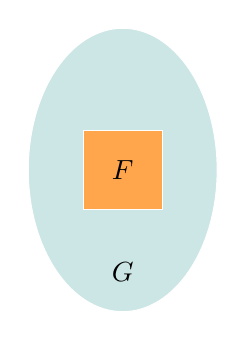
\begin{tikzpicture}
\filldraw[fill=blue!50!green!20, draw=white] (0, 0) ellipse (1.2 and 1.8);
\filldraw[fill=orange!70, draw=white] (-0.5, -0.5) rectangle (0.5, 0.5);
\node at (0, 0) {$F$};
\node at (0, -1.3) {$G$};
\end{tikzpicture}
\hspace{20pt}카테고리 이론(category theory)은 
\hspace{20pt}수학 및 이론 컴퓨터 과학에서 구조들과 그 사이의 관계
\hspace{20pt}들을 연구하는 학문입니다. 카테고리(category)는 객체(objects)와
\hspace{20pt}화살표(arrows 또는 morphisms)로 구성됩니다. 각 화살표는
\hspace{20pt}두 객체 사이를 연결하며, 함수처럼 행동합니다. 
ewline
\hspace{20pt}카테고리는 다음과 같은 구성 요소를 가집니다:
\hspace{20pt}1. 객체들의 모임 \(\mathcal{C}\). 틀린 부분이 그냥 넘어간다.
\hspace{20pt}2. 각 객체 \(X\)와 \(Y\)에 대해, \(X\)에서 \(Y\)로 가는
\hspace{20pt}화살표들의 집합 \(\text{Hom}(X, Y)\).
\hspace{20pt}3. 각 객체 \(X\)에 대해, \(X\)에서 자기 자신으로 가는
\hspace{20pt}항등 화살표(identity arrow) \(\text{id}_X\).
\hspace{20pt}4. 각 세 개의 객체 \(X\), \(Y\), \(Z\)에 대해 두
\hspace{20pt}화살표 \(f \in \text{Hom}(X, Y)\) 및 \(g \in \text{Hom}(Y, Z)\)에 대해
\hspace{20pt}합성 화살표(composite arrow) \(g \circ f \in \text{Hom}(X, Z)\).
ewline
\hspace{20pt}이 합성 연산은 결합 법칙을 만족해야 하며,
\hspace{20pt}모든 객체 \(X\)에 대해 항등원 법칙을 만족해야 합니다:
\hspace{20pt}1. (결합 법칙) 세 개의 화살표 \(f \in \text{Hom}(W, X)\),
\hspace{20pt}\(g \in \text{Hom}(X, Y)\), \(h \in \text{Hom}(Y, Z)\)에 대해,
\hspace{20pt}\(h \circ (g \circ f) = (h \circ g) \circ f\).
\hspace{20pt}2. (항등원 법칙) 모든 화살표 \(f \in \text{Hom}(X, Y)\)에 대해,
\hspace{20pt}\(\text{id}_Y \circ f = f\) 및 \(f \circ \text{id}_X = f\).
ewline
\hspace{20pt}다양한 카테고리의 예로는 집합의 카테고리 \(\textbf{Set}\),
\hspace{20pt}위상 공간의 카테고리 \(\textbf{Top}\), 아벨 군의 카테고리
\hspace{20pt}\(\textbf{Ab}\) 등이 있습니다. 이론 컴퓨터 과학에서는 
\hspace{20pt}프로그래밍 언어의 의미론을 연구하기 위해 카테고리 이론을 사용합니다.
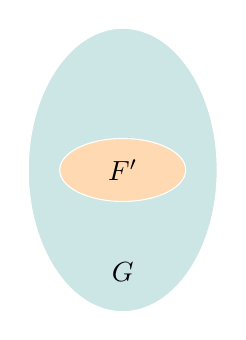
\begin{tikzpicture}
\filldraw[fill=blue!50!green!20, draw=white] (0, 0) ellipse (1.2 and 1.8);
\filldraw[fill=orange!30, draw=white] (0, 0) ellipse (0.8 and 0.4);
\node at (0, 0) {$F'$};
\node at (0, -1.3) {$G$};
\end{tikzpicture}
\hspace{20pt}카테고리 이론(category theory)은 
\hspace{20pt}수학 및 이론 컴퓨터 과학에서 구조들과 그 사이의 관계
\hspace{20pt}들을 연구하는 학문입니다. 카테고리(category)는 객체(objects)와
\hspace{20pt}화살표(arrows 또는 morphisms)로 구성됩니다. 각 화살표는
\hspace{20pt}두 객체 사이를 연결하며, 함수처럼 행동합니다. 
ewline
\hspace{20pt}카테고리는 다음과 같은 구성 요소를 가집니다:
\hspace{20pt}1. 객체들의 모임 \(\mathcal{C}\). 틀린 부분이 그냥 넘어간다.
\hspace{20pt}2. 각 객체 \(X\)와 \(Y\)에 대해, \(X\)에서 \(Y\)로 가는
\hspace{20pt}화살표들의 집합 \(\text{Hom}(X, Y)\).
\hspace{20pt}3. 각 객체 \(X\)에 대해, \(X\)에서 자기 자신으로 가는
\hspace{20pt}항등 화살표(identity arrow) \(\text{id}_X\).
\hspace{20pt}4. 각 세 개의 객체 \(X\), \(Y\), \(Z\)에 대해 두
\hspace{20pt}화살표 \(f \in \text{Hom}(X, Y)\) 및 \(g \in \text{Hom}(Y, Z)\)에 대해
\hspace{20pt}합성 화살표(composite arrow) \(g \circ f \in \text{Hom}(X, Z)\).
ewline
\hspace{20pt}이 합성 연산은 결합 법칙을 만족해야 하며,
\hspace{20pt}모든 객체 \(X\)에 대해 항등원 법칙을 만족해야 합니다:
\hspace{20pt}1. (결합 법칙) 세 개의 화살표 \(f \in \text{Hom}(W, X)\),
\hspace{20pt}\(g \in \text{Hom}(X, Y)\), \(h \in \text{Hom}(Y, Z)\)에 대해,
\hspace{20pt}\(h \circ (g \circ f) = (h \circ g) \circ f\).
\hspace{20pt}2. (항등원 법칙) 모든 화살표 \(f \in \text{Hom}(X, Y)\)에 대해,
\hspace{20pt}\(\text{id}_Y \circ f = f\) 및 \(f \circ \text{id}_X = f\).
ewline
\hspace{20pt}다양한 카테고리의 예로는 집합의 카테고리 \(\textbf{Set}\),
\hspace{20pt}위상 공간의 카테고리 \(\textbf{Top}\), 아벨 군의 카테고리
\hspace{20pt}\(\textbf{Ab}\) 등이 있습니다. 이론 컴퓨터 과학에서는 
\hspace{20pt}프로그래밍 언어의 의미론을 연구하기 위해 카테고리 이론을 사용합니다.
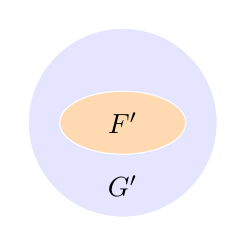
\begin{tikzpicture}
\filldraw[fill=blue!10, draw=white] (0, 0) circle (1.2);
\filldraw[fill=orange!30, draw=white] (0, 0) ellipse (0.8 and 0.4);
\node at (0, 0) {$F'$};
\node at (0, -0.8) {$G'$};
\end{tikzpicture}
\]


혹은 먼저 \hask{beta}를 사용하여 바깥 컨테이너를 다시 포장한 후, \hask{fmap alpha}를 적용하여 모든 내부 컨테이너를 다시 포장할 수 있습니다. 최종 결과는 동일합니다.

\[
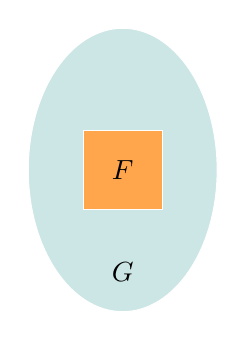
\begin{tikzpicture}
\filldraw[fill=blue!50!green!20, draw=white] (0, 0) ellipse (1.2 and 1.8);
\filldraw[fill=orange!70, draw=white] (-0.5, -0.5) rectangle (0.5, 0.5);
\node at (0, 0) {$F$};
\node at (0, -1.3) {$G$};
\end{tikzpicture}
\hspace{20pt}카테고리 이론(category theory)은 
\hspace{20pt}수학 및 이론 컴퓨터 과학에서 구조들과 그 사이의 관계
\hspace{20pt}들을 연구하는 학문입니다. 카테고리(category)는 객체(objects)와
\hspace{20pt}화살표(arrows 또는 morphisms)로 구성됩니다. 각 화살표는
\hspace{20pt}두 객체 사이를 연결하며, 함수처럼 행동합니다. 
ewline
\hspace{20pt}카테고리는 다음과 같은 구성 요소를 가집니다:
\hspace{20pt}1. 객체들의 모임 \(\mathcal{C}\). 틀린 부분이 그냥 넘어간다.
\hspace{20pt}2. 각 객체 \(X\)와 \(Y\)에 대해, \(X\)에서 \(Y\)로 가는
\hspace{20pt}화살표들의 집합 \(\text{Hom}(X, Y)\).
\hspace{20pt}3. 각 객체 \(X\)에 대해, \(X\)에서 자기 자신으로 가는
\hspace{20pt}항등 화살표(identity arrow) \(\text{id}_X\).
\hspace{20pt}4. 각 세 개의 객체 \(X\), \(Y\), \(Z\)에 대해 두
\hspace{20pt}화살표 \(f \in \text{Hom}(X, Y)\) 및 \(g \in \text{Hom}(Y, Z)\)에 대해
\hspace{20pt}합성 화살표(composite arrow) \(g \circ f \in \text{Hom}(X, Z)\).
ewline
\hspace{20pt}이 합성 연산은 결합 법칙을 만족해야 하며,
\hspace{20pt}모든 객체 \(X\)에 대해 항등원 법칙을 만족해야 합니다:
\hspace{20pt}1. (결합 법칙) 세 개의 화살표 \(f \in \text{Hom}(W, X)\),
\hspace{20pt}\(g \in \text{Hom}(X, Y)\), \(h \in \text{Hom}(Y, Z)\)에 대해,
\hspace{20pt}\(h \circ (g \circ f) = (h \circ g) \circ f\).
\hspace{20pt}2. (항등원 법칙) 모든 화살표 \(f \in \text{Hom}(X, Y)\)에 대해,
\hspace{20pt}\(\text{id}_Y \circ f = f\) 및 \(f \circ \text{id}_X = f\).
ewline
\hspace{20pt}다양한 카테고리의 예로는 집합의 카테고리 \(\textbf{Set}\),
\hspace{20pt}위상 공간의 카테고리 \(\textbf{Top}\), 아벨 군의 카테고리
\hspace{20pt}\(\textbf{Ab}\) 등이 있습니다. 이론 컴퓨터 과학에서는 
\hspace{20pt}프로그래밍 언어의 의미론을 연구하기 위해 카테고리 이론을 사용합니다.
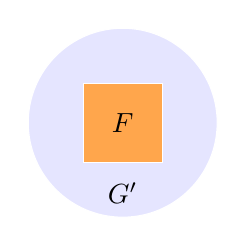
\begin{tikzpicture}
\filldraw[fill=blue!10, draw=white] (0, 0) circle (1.2);
\filldraw[fill=orange!70, draw=white] (-0.5, -0.5) rectangle (0.5, 0.5);
\node at (0, 0) {$F$};
\node at (0, -0.9) {$G'$};
\end{tikzpicture}
\hspace{20pt}카테고리 이론(category theory)은 
\hspace{20pt}수학 및 이론 컴퓨터 과학에서 구조들과 그 사이의 관계
\hspace{20pt}들을 연구하는 학문입니다. 카테고리(category)는 객체(objects)와
\hspace{20pt}화살표(arrows 또는 morphisms)로 구성됩니다. 각 화살표는
\hspace{20pt}두 객체 사이를 연결하며, 함수처럼 행동합니다. 
ewline
\hspace{20pt}카테고리는 다음과 같은 구성 요소를 가집니다:
\hspace{20pt}1. 객체들의 모임 \(\mathcal{C}\). 틀린 부분이 그냥 넘어간다.
\hspace{20pt}2. 각 객체 \(X\)와 \(Y\)에 대해, \(X\)에서 \(Y\)로 가는
\hspace{20pt}화살표들의 집합 \(\text{Hom}(X, Y)\).
\hspace{20pt}3. 각 객체 \(X\)에 대해, \(X\)에서 자기 자신으로 가는
\hspace{20pt}항등 화살표(identity arrow) \(\text{id}_X\).
\hspace{20pt}4. 각 세 개의 객체 \(X\), \(Y\), \(Z\)에 대해 두
\hspace{20pt}화살표 \(f \in \text{Hom}(X, Y)\) 및 \(g \in \text{Hom}(Y, Z)\)에 대해
\hspace{20pt}합성 화살표(composite arrow) \(g \circ f \in \text{Hom}(X, Z)\).
ewline
\hspace{20pt}이 합성 연산은 결합 법칙을 만족해야 하며,
\hspace{20pt}모든 객체 \(X\)에 대해 항등원 법칙을 만족해야 합니다:
\hspace{20pt}1. (결합 법칙) 세 개의 화살표 \(f \in \text{Hom}(W, X)\),
\hspace{20pt}\(g \in \text{Hom}(X, Y)\), \(h \in \text{Hom}(Y, Z)\)에 대해,
\hspace{20pt}\(h \circ (g \circ f) = (h \circ g) \circ f\).
\hspace{20pt}2. (항등원 법칙) 모든 화살표 \(f \in \text{Hom}(X, Y)\)에 대해,
\hspace{20pt}\(\text{id}_Y \circ f = f\) 및 \(f \circ \text{id}_X = f\).
ewline
\hspace{20pt}다양한 카테고리의 예로는 집합의 카테고리 \(\textbf{Set}\),
\hspace{20pt}위상 공간의 카테고리 \(\textbf{Top}\), 아벨 군의 카테고리
\hspace{20pt}\(\textbf{Ab}\) 등이 있습니다. 이론 컴퓨터 과학에서는 
\hspace{20pt}프로그래밍 언어의 의미론을 연구하기 위해 카테고리 이론을 사용합니다.
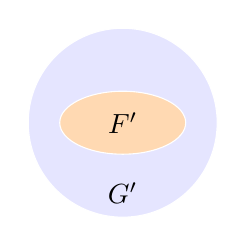
\begin{tikzpicture}
\filldraw[fill=blue!10, draw=white] (0, 0) circle (1.2);
\filldraw[fill=orange!30, draw=white] (0, 0) ellipse (0.8 and 0.4);
\node at (0, 0) {$F'$};
\node at (0, -0.9) {$G'$};
\end{tikzpicture}
\]


\begin{exercise}
Implement two versions of horizontal composition of \hask{safeHead} after \hask{reverse}. Compare their results acting on various arguments.
\end{exercise}

\begin{exercise}
Do the same with the horizontal composition of \hask{reverse} after \hask{safeHead}. 
\end{exercise}

\subsection{휘스커링(Whiskering)}

대개 수평 합성은 하나의 자연 변환이 항등 변환(identity)일 때 사용됩니다. 이러한 합성에 대한 축약 표시법이 있습니다. 예를 들어, $\alpha \circ id_F$는 $\alpha \circ F$로 씁니다.

그 그림의 특징적인 모양 때문에, 그러한 합성은 ``수염달기(whiskering)''라고 불립니다.
\[
\begin{tikzcd}[column sep=huge]
\mathcal{C}
 \arrow[r, "F"]
 &
\mathcal{D}
  \arrow[bend left=50]{r}[name=U1, label=above:$G$]{}
  \arrow[bend right=50]{r}[name=D1, label=below:$G'$]{} 
 &
\mathcal{E}
  \arrow[shorten <=10pt,shorten >=10pt,Rightarrow,to path={(U1) -- node[label=left:$\alpha$] {} (D1)}]{}
\end{tikzcd}
\]
구성 요소 별로, 우리는 가지고 있습니다:
\[ (\alpha \circ F)_x = \alpha_{F x} \]

Haskell로 이를 어떻게 번역할지 생각해 봅시다. 자연 변환(natural transformation)은 다형 함수(polymorphic function)입니다. 매개변수 적합성(parametricity)의 특성상, 이는 모든 유형에 대해 동일한 공식으로 정의됩니다. 그러므로 오른쪽에서의 '휘지기(whiskering)'는 공식을 바꾸지 않고, 함수 시그니처를 바꿉니다.

예를 들어, 이것이 \hask{alpha}의 선언이라면:
\begin{haskell}
alpha :: forall x. G x -> G' x
\end{haskell}
그러면 그것의 수염달린(whiskered) 버전은 다음과 같을 것이다:
\begin{haskell}
alpha_f :: forall x. G (F x) -> G' (F x)
alpha_f = alpha
\end{haskell}
Haskell의 타입 추론(type inference) 덕분에, 이 전환은 암묵적입니다. 다형성 함수(polymorphic function)가 호출될 때, 우리는 자연 변환(natural transformation)의 어떤 구성 요소가 실행되는지 명시할 필요가 없습니다--타입 검사기(type checker)가 인자의 타입을 보고 알아냅니다.

직관적으로 이 경우 외부 컨테이너를 재포장하고 내부 컨테이너는 그대로 두는 것입니다.

마찬가지로, $id_H \circ \alpha$는 $H \circ \alpha$로 쓰입니다.
\[
\begin{tikzcd}[column sep=huge]
\mathcal{D}
  \arrow[bend left=50]{r}[name=U, label=above:$G$]{}
  \arrow[bend right=50]{r}[name=D, label=below:$G'$]{} 
 &
\mathcal{E}
\arrow[r, "H"]
&
\mathcal{F}
  \arrow[shorten <=10pt,shorten >=10pt,Rightarrow,to path={(U) -- node[label=left:$\alpha$] {} (D)}]{}
\end{tikzcd}
\]
구성 요소들에 있어:
\[(H \circ \alpha)_x = H (\alpha_x) \]

Haskell에서, $\alpha_x$를 $H$로 들어올리는 작업은 \hask{fmap}을 사용하여 수행됩니, 그래서 주어진 경우:
\begin{haskell}
alpha :: forall x. G x -> G' x
\end{haskell}
수염 달린 버전은 다음과 같을 것입니다:
\begin{haskell}
h_alpha :: forall x. H (G x) -> H (G' x)
h_alpha = fmap alpha
\end{haskell}
다시 말해, Haskell의 타입 추론 엔진(type inference engine)은 어느 버전의 \hask{fmap}을 사용할지 결정합니다 (여기서는 \hask{G}의 \hask{Functor} 인스턴스에서 온 것입니다).

직관은 외부 용기를 그대로 둔 채 내부 용기의 내용을 다시 포장하고 있다는 것입니니다.

드디어, 많은 응용에서 자연 변환(natural transformation)은 양쪽에서 휘파람을 맞춥니다:
\[
\begin{tikzcd}[column sep=huge]
\mathcal{C}
 \arrow[r, "F"]
 &
\mathcal{D}
  \arrow[bend left=50]{r}[name=U1, label=above:$G$]{}
  \arrow[bend right=50]{r}[name=D1, label=below:$G'$]{} 
 &
\mathcal{E}
  \arrow[shorten <=10pt,shorten >=10pt,Rightarrow,to path={(U1) -- node[label=left:$\alpha$] {} (D1)}]{}
  \arrow[r, "H"]
 &
 \mathcal{F}
\end{tikzcd}
\]
구성 요소 별로, 우리는 가지고 있습니다:
\[ (H \circ \alpha \circ F) x = H (\alpha_{F x})\]
그리고 Haskell에서:
\begin{haskell}
h_alpha_f :: forall x. H (G (F x)) -> H (G' (F x))
h_alpha_f = fmap alpha
\end{haskell}

여기서 직관적으로 이해할 수 있는 것은 우리가 세 겹의 컨테이너(용기)를 가지고 있다는 것이며, 중간 컨테이너를 재배치하고 바깥 컨테이너와 모든 내부 컨테이너는 그대로 둔다는 것입니다.

\subsection{교환 법칙 (Interchange law)}

우리는 아래 도표에서 볼 수 있듯이 수직 합성과 수평 합성을 결합할 수 있습니다:
\[
\begin{tikzcd}[column sep=huge]
\mathcal{C}
  \arrow[bend left=60]{rr}[name=U, label=above:$F$]{}
  \arrow[]{rr}[name=M, label={[xshift=15pt, yshift=-5pt]:$G$}]{} 
  \arrow[bend right=60]{rr}[name=D, label=below:$H$]{} 
 &&
\mathcal{D}
  \arrow[bend left=60]{rr}[name=U1, label=above:$F'$]{}
  \arrow[]{rr}[name=M1, label={[xshift=15pt, yshift=-5pt]:$G'$}]{} 
  \arrow[bend right=60]{rr}[name=D1, label=below:$H'$]{} 
&&
\mathcal{E}
  \arrow[shorten <=8pt, shorten >=8pt,Rightarrow, to path={(U) -- node[label=left:$\alpha$] {} (M)}]{}
  \arrow[shorten <=8pt, shorten >=8pt,Rightarrow, to path={(M) -- node[label=left:$\beta$] {} (D)}]{}
  \arrow[shorten <=8pt, shorten >=8pt,Rightarrow, to path={(U1) -- node[label=left:$\alpha'$] {} (M1)}]{}
  \arrow[shorten <=8pt, shorten >=8pt,Rightarrow, to path={(M1) -- node[label=left:$\beta'$] {} (D1)}]{}
\end{tikzcd}
\]
교환 법칙은 합성의 순서가 중요하지 않음을 나타냅니다: 먼저 수직 합성을 하고 가로 합성을 하거나, 먼저 가로 합성을 하고 수직 합성을 할 수 있습니다.


\section{보편적 구성 다시 보기}

노자(Lao Tzu)는 말합니다, 가장 단순한 패턴이 가장 명확합니다.

우리는 합(sum), 곱(product), 지수(exponentials), 자연수(natural numbers), 그리고 리스트(lists)의 정의를 보았습니다.

예전 방식으로 이러한 데이터 타입을 정의하는 접근법은 그것들의 내부를 탐구하는 것입니다. 이것은 집합 이론(set-theory) 방식입니다: 우리는 새로운 집합의 요소들이 어떻게 기존 집합의 요소들로부터 구성되는지 살펴봅니다. 합집합의 요소는 첫 번째 집합의 요소이거나 두 번째 집합의 요소입니다. 곱집합의 요소는 요소들의 쌍(pair)입니다. 그리고 계속해서. 우리는 공학 관점에서 객체들을 바라보고 있습니다.

카테고리 이론(category theory)에서는 반대 접근 방식을 취합니다. 객체(object) 내부에 무엇이 있는지 또는 그것이 어떻게 구현되었는지에는 관심이 없습니다. 우리는 객체의 목적, 그것이 어떻게 사용될 수 있는지, 그리고 다른 객체들과 어떻게 상호작용하는지에 관심이 있습니다. 우리는 유용성(utilitarian) 관점에서 객체를 살펴봅니다.

두 접근 방식 모두 장점이 있습니 다. 범주론적 접근 방식(categorical approach)은 나중에 등장했는데, 이는 명확한 패턴이 드러나기 전에 많은 예제를 공부할 필요가 있기 때문입니 다. 하지만 일단 패턴을 이해하게 되면, 합(sum)과 곱(product) 사이의 이중성(duality)과 같은 예상치 못한 연결고리를 발견할 수 있습니 다.

특정 객체를 그들의 연결을 통해 정의하기 위해서는 그들이 상호작용하는 무한한 수의 객체를 살펴봐야 할 수 있습니다.

``당신의 우주와의 관계를 말해 주세요. 그러면 제가 당신이 누구인지 알려드릴게요.''

모든 사물과의 매핑 아웃 또는 매핑 인에 의해 사물을 정의하는 것을 \emph{보편적 구성}(universal construction)이라 합니다.

왜 자연 변환(natural transformations)이 그렇게 중요합니까? 그것은 대부분의 범주론적 구성들이 교환 다이어그램(commuting diagrams)을 포함하기 때문입니다. 만약 이 다이어그램들을 자연성 사각형(naturality squares)으로 다시 표현할 수 있다면, 우리는 추상화 단계의 한 단계를 더 올라 새로운 귀중한 통찰을 얻을 수 있습니다.

많은 사실들을 작은 우아한 공식들로 압축할 수 있다는 것은 새로운 패턴을 볼 수 있게 해줍니다. 
예를 들어, hom-집합들 사이의 자연스러운 동형사상(natural isomorphisms)이 범주 이론(category theory)의 여러 곳에서 나타나고 
결국 사상(adjunction)의 개념으로 이어진다는 것을 보게 될 것입니다.

하지만 먼저 우리는 범주론(category theory)의 간결한 언어를 이해하기 위해 몇 가지 예제를 자세히 연구할 것입니다. 예를 들어, 두 객체(object)의 합(coproduct), 또는 쌍대곱이 다음과 같은 자연동형사상(natural isomorphism)에 의해 정의된다는 명제를 해독해 보겠습니다:

\[ [\mathbf{2}, \mathcal{C}](D, \Delta_x)  \cong \mathcal{C}(a + b, x) \]



\subsection{객체 선택}

심지어 어떤 물체를 가리키는 것과 같은 단순한 작업도 범주 이론(category theory)에서는 특별한 해석이 있습니. 우리는 이미 집합의 요소를 가리키는 것이 그 집합으로 향하는 단일 원소 집합의 함수(function)를 선택하는 것과 동등하다는 것을 보았습니. 마찬가지로, 범주에서 객체를 선택하는 것은 단일 객체 범주에서의 함자(functor)를 선택하는 것과 동등합니. 또는 다른 범주에서의 상수 함자를 이용하여 수행할 수 있습니.

때때로 우리는 한 쌍의 객체(object)를 선택하고 싶습니다. 이것 역시 두 객체로 구성된 단순한 범주(category)에서 함자(functor)를 선택함으로써 달성할 수 있습니다. 유사하게, 화살(arrow)을 선택하는 것은 "걸어다니는 화살"(walking arrow) 범주에서 함자를 선택하는 것과 동일합니다, 그리고 계속해서 말입니다.

우리의 함자(functors)와 그들 사이의 자연 변환(natural transformations)을 신중하게 선택함으로써 이제까지 본 모든 보편적 구성(universal constructions)을 재구성할 수 있습니다.

\subsection{코스팬(cospan)들을 자연 변환(natural transformation)으로서}

합의(definition of a sum) 정의는 더할 두 개의 객체(object)를 선택하는 것과 매핑(mapping) 결과의 대상이 될 세 번째 객체를 선택하는 것을 필요로 합니다.

\[
 \begin{tikzcd}
 a
 \arrow[dr,  bend left, "\text{Left}"']
 \arrow[ddr, bend right, "f"']
 && b
 \arrow[dl, bend right, "\text{Right}"]
 \arrow[ddl, bend left, "g"]
 \\
&a + b
\arrow[d, dashed, "h"]
\\
& c
 \end{tikzcd}
\]
이 도표(diagram)는 \emph{공간들(cospans)}이라고 불리는 더 간단한 두 개의 형태로 다시 나눌 수 있습니다:
\[
 \begin{tikzcd}
 a
 \arrow[dr, ""']
 && b
 \arrow[dl, ""]
 \\
 & x
 \end{tikzcd}
\]

먼저 코스팬(cospan)을 구성하려면 객체(pair of objects)를 선택해야 합니다. 이를 위해 두 객체의 범주(category) $\mathbf{2}$를 시작점으로 하겠습니다. 객체들은 $1$과 $2$라고 부르겠습니다.
펑터(functor)를 사용합니다
\[ D \colon \mathbf{2} \to \mathcal{C}\]
객체 $a$와 $b$를 선택하려면:
\begin{align*}
D\, 1 &= a \\
D\, 2 &= b 
\end{align*}
($D$는 ``다이어그램''을 나타냅니다. 두 개의 객체가 $\mathcal{C}$에서 두 개의 점으로 구성된 매우 단순한 다이어그램을 형성하기 때문입니다.)

상수 함자(constant functor)를 사용하겠습니
\[ \Delta_x \colon \mathbf{2} \to \mathcal{C} \]
객체 $x$를 선택하기 위해서입니다. 이 함자는 $1$과 $2$ 모두를 $x$로 매핑합니다 (그리고 두 개의 항등 사상을 $id_x$로 매핑합니다).

둘 다 함자(functors)가 $\mathbf{2}$에서 $\mathcal{C}$로 가므로, 그 사이에 자연 변환(natural transformation) $\alpha$를 정의할 수 있습니다. 이 경우, 그것은 한 쌍의 화살표일 뿐입니다:
\begin{align*}
\alpha_1 \colon D \, 1 \to \Delta_x 1 \\
\alpha_2 \colon D \, 2 \to \Delta_x 2
\end{align*}
이것들은 공동체(span)에 있는 정확히 두 개의 화살표입니다.

$\alpha$에 대한 자연성 조건(naturality condition)은 자명합니다, 왜냐하면 $\mathbf{2}$에는 (동일성 이외의) 화살표가 없기 때문입니다.

많은 코스판(cospan)이 동일한 세 개의 객체를 공유할 수 있습니다. 이는 두 함자(functor) $D$와 $\Delta_x$ 사이에 많은 자연 변환(natural transformation)이 있을 수 있다는 것을 의미합니다. 이러한 자연 변환들은 함자 범주(functor category) $[\mathbf{2}, \mathcal{C}]$에서 하나의 동형사상 집합(hom-set)을 이루며, 즉:
\[ [\mathbf{2}, \mathcal{C}](D, \Delta_x) \]

\subsection{코스팬의 함자성(Functoriality of cospans)}

$x$의 물체(object)를 코스팬(cospan)에서 변형하기 시작할 때 어떤 일이 일어나는지 생각해 봅시다. 우리는 $x$를 코스팬들의 집합으로 매핑하는 매핑 $F$를 가지고 있습니다:
\[ F x = [\mathbf{2}, \mathcal{C}](D, \Delta_x) \]
이 사상(mapping)은 $x$에 대해서 함자적(functorial)입니다.

이를 보기 위해, 화살표 $m \colon x \to y$를 고려합니다. 이 화살표의 리프팅(lifting)은 두 자연 변환 집합 사이의 매핑(mapping)입니다:
\[ [\mathbf{2}, \mathcal{C}](D, \Delta_x) \to [\mathbf{2}, \mathcal{C}](D, \Delta_{y}) \] 
 
이것은 자연 변환(natural transformations)이 구성 요소를 가지고 있으며, 이 구성 요소들이 단순한 일반 화살표라는 것을 기억하면 매우 추상적으로 보일 수 있습니니다. 왼쪽 항의 하나의 요소는 자연 변환입니니다:
\[ \mu \colon D \to \Delta_x \]
두 개체(objects)를 나타내는 두 구성 요소(component)를 가지고 있습니다. 예를 들어, 우리는
\[ \mu_1 \colon D \, 1 \to \Delta_x 1 \]
또는, $D$와 $\Delta$의 정의(Definitions)를 사용하여:
\[ \mu_1 \colon a \to x \]
이것은 우리의 코스팬(cospan)의 왼쪽 다리일 뿐입니다.

동일하게, 오른쪽 항의 원소는 자연 변환(natural transformation)입니다:
\[ \nu \colon D \to \Delta_{y} \]
그 내용물 중 $1$에 해당하는 것은 화살표(arrow)입니다.
\[ \nu_1 \colon a \to y \]
$\mu_1$에서 $u_1$로 가려면 단순히 $m \colon x \to y$와 함께 뒤에 합성하면 됩니다. 따라서 $m$의 올림은 각 구성 요소별 후 합성 $(m \circ -)$입니다:
\begin{align*}
\nu_1 = m \circ \mu_1 \\
\nu_2 = m \circ \mu_2 \\
\end{align*}

\subsection{합(함(sum))이 보편적인 코스팬(cospan)임}

모든 cospan들 중 $a$와 $b$ 쌍에 대해 만들 수 있는 것들 중에서, 화살표 $\text{Left}$와 $\text{Right}$가 $a + b$로 수렴하는 것이 매우 특별합니다. 이 cospan에서 다른 어떤 cospan으로의 유일한 매핑(mapping)이 존재합니다---이는 두 삼각형을 움직이게(commute) 만드는 매핑입니다.
\[
 \begin{tikzcd}
 a
 \arrow[dr,  bend left, "\text{Left}"']
 \arrow[ddr, bend right, "f"']
 && b
 \arrow[dl, bend right, "\text{Right}"]
 \arrow[ddl, bend left, "g"]
 \\
&a + b
\arrow[d, dashed, "h"]
\\
& x
 \end{tikzcd}
\]

이제 우리는 이 조건을 자연 변환(natural transformations)과 사상 집합(hom-sets)에 대한 진술로 번역할 수 있는 위치에 있습니다. 화살표 $h$는 사상 집합의 요소입니다
\[ \mathcal{C}(a + b, x)\]
$x$ 위의 코스팬(cospan)은 자연 변환(natural transformation)이고, 이는 펑터 범주(functor category)에서의 hom-집합의 원소를 의미합니다:
\[ [\mathbf{2}, \mathcal{C}](D, \Delta_x) \]

둘 다 각자의 범주에서의 hom-셋(hom-sets)입니다. 그리고 둘 다 단순히 집합, 즉 범주 $\mathbf{Set}$의 객체(object)들입니다. 이 범주는 함자 범주(functor category) $[\mathbf{2}, \mathcal{C}]$와 ``일반" 범주 $\mathcal{C}$ 사이의 다리를 형성합니다. 비록 개념적으로는, 이들이 매우 다른 추상화 수준에 있는 것처럼 보일지라도 말입니다.

지그문트 프로이트를 패러프레이징(Paraphrasing)하면, ``때로는 집합(set) 은 그저 집합일 뿐이다.''

우리의 보편적 구성은 집합의 전단사(또는 동형사상(isomorphism))입니다:
\[ [\mathbf{2}, \mathcal{C}](D, \Delta_x)  \cong \mathcal{C}(a + b, x) \]

게다가, 객체 $x$를 변경하면, 두 측면은 $\mathcal{C}$에서 $\mathbf{Set}$으로 가는 함자처럼 동작합니다. 따라서 이 함자들의 매핑이 자연동형사상(natural isomorphism)인지 묻는 것이 합리적입니다.

실제로, 이 동형사상(naturality condition for this isomorphism)의 자연성 조건이 합(sum)의 정의에서 삼각형들의 교환 조건으로 변환된다는 것을 보일 수 있습니 다. 따라서 합의 정의는 단일한 하나의 방정식으로 대체될 수 있습니다.

\subsection{곱(Product)으로서의 일반적 퍼짐(Universal Span)}

유사한 논증을 곱(product)의 범주의 보편적인 구성(construction)으로 만들 수 있습니다. 이번에도 막대 그림 범주(stick-figure category) $\mathbf{2}$와 함자(functor) $D$로 시작합니다. 하지만 이번에는 반대 방향으로 가는 자연 변환(natural transformation)을 사용합니다.
\[ \alpha \colon \Delta_x \to D \]
그러한 자연 변환은 \emph{span}(스팬)을 형성하는 한 쌍의 화살표입니다:
\[
 \begin{tikzcd}
 &x
 \arrow[dl, "f"']
 \arrow[dr, "g"]
 \\
 a
 && b
  \end{tikzcd}
\]
집합적으로, 이러한 자연 변환들은 함자 범주에서 하나의 hom-집합(hom-set)을 이룹니다:
\[[\mathbf{2}, \mathcal{C}](\Delta_x, D) \]

이 hom-집합의 모든 요소는 유일한 사상 $h$와 일대일 대응됩니다. 이 사상은 곱 $a \times b$로의 사상 집합 $\mathcal{C}(x, a \times b)$의 멤버입니다. 이 대응은 다음과 같은 동형사상으로 표현됩니다:
\[ [\mathbf{2}, \mathcal{C}](\Delta_x, D)  \cong \mathcal{C}(x, a \times b) \]
이 동형사상이 자연적이라는 것은 이 도형의 삼각형들이 가환함을 보장함을 증명할 수 있~니다.

\[
 \begin{tikzcd}
 & C 
\arrow[d, dashed, "h"]
 \arrow[ddl, bend right, "f = \alpha_1"']
 \arrow[ddr, bend left, "g = \alpha_2"]
\\
&a \times b
 \arrow[dl,  "\text{fst}"]
  \arrow[dr,   "\text{snd}"']
\\
a = D\, 1 && b = D \, 2
 \end{tikzcd}
\]

\subsection{지수(Exponentials)}

지수, 또는 함수 객체(function objects), 는 이 교환 다이어그램(commuting diagram)에 의해 정의됩니다.
\[
 \begin{tikzcd}
 x \times a
 \arrow[d, dashed, "h \times id_a"']
 \arrow[rd, "f"]
 \\
 b^a \times a
 \arrow[r, "\varepsilon_{a b}"']
& b
 \end{tikzcd}
\]
여기서 $f$는 동형사상 모임(hom-set) $\mathcal{C}(x \times a, b)$의 원소이고 $h$는 $\mathcal{C}(x, b^a)$의 원소입니다.

이들 집합 사이의 동형(isomorphism), $x$에서의 자연성(natural) 속에서, 지수 대상(exponential object)을 정의해 줍니다.
\[\mathcal{C}(x \times a, b) \cong \mathcal{C}(x, b^a)\]

다이어그램 위의 $f$는 왼쪽의 원소이며, $h$는 오른쪽에 해당하는 원소입니다. 변환 $\alpha_x$ (이는 $a$ 및 $b$에도 의존함)는 $f$를 $h$로 매핑합니다.
\[ \alpha_x \colon \mathcal{C}(x \times a, b) \to \mathcal{C}(x, b^a) \]
In Haskell, 우리는 그것을 \hask{curry}라고 부릅니다. 그 역함수 $\alpha^{-1}$는 \hask{uncurry}로 알려져 있습니다.

이전 예제와는 달리, 여기서는 두 hom-집합이 같은 범주(category) 안에 있으며, 동형사상(isomorphism)을 더 자세히 분석하는 것이 쉽습니다. 특히, 우리는 다음과 같은 통근 조건(commuting condition)이 어떻게 되는지 보고 싶습니다:
\[  f = \varepsilon_{a b} \circ (h \times id_a) \]
자연스러움에서 발생합니다.

표준 요네다 기법은 $x$에 대한 대체를 통해 하나의 hom-집합을 endo-hom-집합으로 줄이는 것입니다. 즉, 시작점과 목표점이 같은 hom-집합으로 만드는 것입니다. 이는 해당 hom-집합의 정식 요소인 항등 화살표(identity arrow)를 선택할 수 있게 해줍니다.

우리의 경우, $b^a$를 $x$로 대체하면 $h = id_{(b^a)}$를 선택할 수 있습니다.
\[
 \begin{tikzcd}
 b^a \times a
 \arrow[d, dashed, "id_{(b^a)} \times id_a"']
 \arrow[rd, "f"]
 \\
 b^a \times a
 \arrow[r, "\varepsilon_{a b}"']
& b
 \end{tikzcd}
\]
이 경우의 교환 조건은 $f = \varepsilon_{a b}$임을 알려줍니다. 다시 말해, $\alpha$에 대한 $\varepsilon_{a b}$의 공식을 얻게 됩니다:
\[ \varepsilon_{a b} = \alpha_{x}^{-1} (id_{x}) \]
여기서 $x$는 $b^a$와 같습니다.

우리가 $\alpha^{-1}$을 \hask{uncurry}로 인식하고, $\varepsilon$을 함수 응용(function application)으로 인식하기 때문에, 이를 Haskell로 다음과 같이 쓸 수 있습니:
\begin{haskell}
apply :: (a -> b, a) -> b
apply = uncurry id
\end{haskell}
처음에는 이것이 놀라울 수 있지만, \hask{(a->b,a)->b}의 커링(currying)이 \hask{(a->b)->(a->b)}로 이어진다는 것을 깨달을 때까지입니다.

우리는 주요 동형사상(isomorphism)의 양쪽을 Haskell 함자(functor)로도 인코딩할 수 있습니다:
\begin{haskell}
data LeftFunctor  a b x = LF ((x, a) -> b)
\end{haskell}
\begin{haskell}
data RightFunctor a b x = RF (x -> (a -> b))
\end{haskell}
그들은 \hask{x} 타입 변수에서 둘 다 반변 수반 함자(contravariant functors)입니다.
\begin{haskell}
instance Contravariant (LeftFunctor a b) where
  contramap g (LF f) = LF (f . bimap g id)
\end{haskell}
이것은 $g \colon x \to y$의 올림이 다음과 같은 사전 구성에 의해 주어진다는 것을 말합니다:
\[ \mathcal{C}(y \times a, b) \xrightarrow{(- \circ (g \times id_a)) }  \mathcal{C}(x \times a, b)\]

비슷하게:
\begin{haskell}
instance Contravariant (RightFunctor a b) where
  contramap g (RF h) = RF (h . g)
\end{haskell}
다음과 같은 가정 가설이 있다. $(X, \tau_X)$와 $(Y, \tau_Y)$가 위상 공간이고 $f: X \to Y$가 함수라 가정하자.
이러한 함수 $f$가 연속(continuous)임을 보여야 한다.
$U$가 $\tau_Y$에 속하는 열린 집합(open set)이라면 $f^{-1}(U)$가 $\tau_X$에 속하는 열린 집합임을 보여야 한다.
\[  \mathcal{C}(y, b^a) \xrightarrow{ (- \circ g) } \mathcal{C}(x, b^a) \]

자연 변환 $\alpha$는 \hask{curry}의 얇은 캡슐화일 뿐입니다; 그리고 그 역함수는 \hask{uncurry}입니다:

\begin{haskell}
alpha :: forall a b x. LeftFunctor a b x -> RightFunctor a b x
alpha (LF f) = RF (curry f)
\end{haskell}

\begin{haskell}
alpha_1 :: forall a b x. RightFunctor a b x -> LeftFunctor a b x
alpha_1 (RF h) = LF (uncurry h)
\end{haskell}

$g \colon x \to y$의 올림에 대한 두 공식을 사용하여, 다음은 자연성 사각형입니다:

\[
 \begin{tikzcd}
 \mathcal{C}(y \times a, b)
 \arrow[rr, "(- \circ (g \times id_a))"]
 \arrow[d,  "\alpha_y"]
& &
\mathcal{C}(x \times a, b)
  \arrow[d, "\alpha_x"]
 \\
 \mathcal{C}(y, b^a)
 \arrow[rr, "(- \circ g)"]
& &
\mathcal{C}(x, b^a)
 \end{tikzcd}
\]

이제 요네다 트릭(Yoneda trick)을 적용해서 $y$를 $b^a$로 대체해 보겠습니다. 이는 또한 $g$를 대체할 수 있게 해줍니다---이는 이제 $x$에서 $b^a$로 가도록 변합니다---$h$로.

\[
 \begin{tikzcd}
 \mathcal{C}(b^a \times a, b)
 \arrow[rr, "(- \circ (h \times id_a))"]
 \arrow[d,  "\alpha_{(b^a)}"]
& &
\mathcal{C}(x \times a, b)
  \arrow[d,  "\alpha_x"]
 \\
 \mathcal{C}(b^a, b^a)
 \arrow[rr, "(- \circ h)"]
& &
\mathcal{C}(x, b^a)
 \end{tikzcd}
\]

우리는 hom-집합 $\mathcal{C}(b^a, b^a)$가 최소한 항등 화살표를 포함하고 있음을 알고 있으므로, 좌측 하단 모서리에 $id_{(b^a)}$ 원소를 선택할 수 있습니다.

화살표를 왼쪽으로 반전시키면, $\alpha^{-1}$가 항등원에 작용하여 왼쪽 위 모서리에 $\varepsilon_{a b}$를 생성한다는 것을 압니다 (이것이 \hask{uncurry id} 트릭입니다).

$h$ 와 함께 전치를 수행하면 식별자가 오른쪽 아래에 $h$를 생성합니다.

$\alpha^{-1}$이 $h$에 작용하여 오른쪽 위 모서리에 $f$를 생성합니다.

\[
 \begin{tikzcd}[
  every arrow/.style={draw,mapsto}
]
 \varepsilon_{a b}
 \arrow[rr, "(- \circ (h \times id_a))"]
& &
f
 \\
 id_{(b^a)}
 \arrow[u, "\alpha^{-1}"]
 \arrow[rr, "(- \circ h)"]
& &
h
\arrow[u, "\alpha^{-1}"']
 \end{tikzcd}
\]
(The $\mapsto$ 화살표는 집합의 원소에 대한 함수의 작용을 나타냅니다.)


그래서 왼쪽 아래 모서리에서 $id_{(b^a)}$의 선택이 나머지 세 모서리를 고정시킵니다. 특히, 우리는 상단 화살표가 $\varepsilon_{a b}$에 적용되어 $f$를 생성하는 것을 볼 수 있는데, 이것은 정확히 그 상환 조건(commuting condition)입니다:
\[ \varepsilon_{a b} \circ (h \times id_a) = f \]
우리가 도출하기로 한 것.

\section{극한(Limits)과 쌍대극한(Colimits)}

이전 섹션에서는 자연변환(natural transformations)을 사용하여 합(sum)과 곱(product)을 정의하였습니다. 이들은 매우 단순한 막대기 도형 카테고리인 $\mathbf{2}$에서 함자로 정의된 도표들 사이의 변환들이었으며, 그 중 하나의 함자는 상수 함자(constant functor)였습니다.

우리를 카테고리 $\mathbf{2}$를 더 복잡한 것으로 대체하는 것을 막는 것은 없습니다. 예를 들어, 우리는 객체들 사이에 비자명한 화살표(non-trivial arrows)가 있는 카테고리나 무한히 많은 객체가 있는 카테고리를 시도해 볼 수 있습니다.

그러한 구성(구조)들에 관한 전체의 용어(어휘)가 있습니다.

우리는 범주 $\mathbf{2}$의 객체들을 범주 $\mathcal{C}$의 객체들을 색인하는 데 사용하였습니다. 우리는 $\mathbf{2}$를 임의의 색인 범주 $\cat J$로 대체할 수 있습니다. $\mathcal{C}$에서의 다이어그램(diagram)은 여전히 함자 $D \colon \cat J \to \mathcal{C}$로 정의됩니다. 이는 $\mathcal{C}$의 객체들을 선택할 뿐만 아니라 그 객체들 사이의 몇몇 화살들도 선택합니다.

두 번째 함자(functor)로 상수 함자(constant functor) $\Delta_x \colon \cat J \to \mathcal{C}$을(를) 여전히 사용할 예정입니다.

자연 변환(natural transformation)은 hom-셋(hom-set)의 원소입니다.
\[ [\cat J, \mathcal{C}](\Delta_x, D)  \]
is now called a \emph{원뿔}(cone)입니다. 그것의 쌍대는,
\[ [\cat J, \mathcal{C}](D, \Delta_x)  \]
를 \emph{코콘}(cocone)이라고 합니다. 이는 각각 스팬(span)과 코스팬(cospan)을 일반화합니다.

도식적으로, 원뿔(cones)과 쌍대원뿔(cocones)은 다음과 같습니다:
\[
 \begin{tikzcd}
  & x
\arrow[ddr, "g"]
 \arrow[ddl, "f"']
 \arrow[ddd, "h"]
 \\
\\
D 1 
\arrow[rr, red]
\arrow[rd, red]
&& D 2
\arrow[dl, red]
\\
& D 3
 \end{tikzcd}
\qquad

카테고리 이론(category theory)에 대한 상당수의 연구는
일반적인 대수적 구조(algebraic structures)를 추상적으로 탐구하는 것에 초점을 둡니다.
우리는 이러한 구조들을
범주(category)라고 부르며,
이러한 범주의 예시로는 집합(set), 군(group), 능환(ring), 모노이드(monoid) 등이 있습니다.
범주는 객체(object)와 사상(morphism)으로 구성됩니다.
각 객체 \(A, B, C, \ldots\)에 대해 사상 \(f: A \rightarrow B\), \(g: B \rightarrow C\) 등이 있습니다.
이 사상들은 합성(composition)과 항등(identity) 연산을 만족해야 합니다\ldots

범주 \(\mathcal{C}\)에서
모든 두 객체 \(A\)와 \(B\) 사이에는 사상의 모음 \(\hom_{\mathcal{C}}(A, B)\)이 존재합니다.
사상의 합성은 결합 법칙(결합 법칙: 영문 필요시: associativity)을 만족합니다.
즉, 모든 \(f: A \rightarrow B\), \(g: B \rightarrow C\), \(h: C \rightarrow D\)에 대해,
\[ h \circ (g \circ f) = (h \circ g) \circ f \]
가 성립합니다.
또한, 각 객체 \(A\)에 대해
항등 사상 \( \operatorname{id}_A: A \rightarrow A \)가 존재하여,
각 사상 \(f: A \rightarrow B\)와 \(g: B \rightarrow A\)에 대해
\[ \operatorname{id}_B \circ f = f \quad \text{와} \quad g \circ \operatorname{id}_B = g \]
가 성립합니다.

모노이드(monoid)는 하나의 객체로 이루어진 범주와 같습니다.
이때, 사상은 모노이드의 원소이며, 사상의 합성은 모노이드 연산입니다.
예를 들어, 정수의 집합 \((\mathbb{Z}, +, 0)\)는 모노이드입니다.
범주는 또한 다른 범주 간의 구조적 관계를 연구할 수 있습니다.
펑터(functor)는 범주 사이의 사상입니다.
\begin{itemize}
\item 하나의 범주 \(\mathcal{C}\)에서 다른 범주 \(\mathcal{D}\)로 가는 펑터 \(F\)는 각 객체 \(A \in \mathcal{C}\)에 \(\mathcal{D}\)의 객체 \(F(A)\)를 대응시키고,
각 사상 \(f: A \rightarrow B\)에 \(\mathcal{D}\)의 사상 \(F(f): F(A) \rightarrow F(B)\)를 대응시킵니다.
\end{itemize}


펑터는 합성 및 항등 사상을 보존합니다.
즉,
\[
F(\operatorname{id}_A) = \operatorname{id}_{F(A)} \quad \text{와} \quad F(g \circ f) = F(g) \circ F(f) \]
가 성립합니다.
이러한 의미에서 펑터는 범주 간의 구조를 보존하는 매핑을 제공합니다.
위를 요약하자면, 카테고리 이론은 수학의 다양한 분과를
통합하고 추상화할 수 있는 강력한 도구를 제공합니다.

다음으로는 자연변환(natural transformation)에 대해 설명하겠습니다.
자연변환은 두 펑터 사이의 사상입니다.
예를 들어, 두 펑터 \(F, G: \mathcal{C} \rightarrow \mathcal{D}\)가 존재합니다.
\begin{tikzcd}
 D 1
 \arrow[rr, red]
 \arrow[dr, red]
 \arrow[dddr, "f"']
 && D 2
\arrow[dl, red]
 \arrow[dddl, "g"]
 \\
 & D 3
 \arrow[dd, "h"]
 \\
 \\
 & x
 \end{tikzcd}
 \]

지표 범주(indexing category)에 이제 화살표(arrows)가 포함될 수 있으므로, 이러한 도표(diagrams)에 대한 자연성 조건들은 더 이상 자명하지 않읍니다. 상수 함자(functor) $\Delta_x$는 모든 꼭짓점(vertices)을 하나로 축소시키므로, 자연성 사각형(naturality squares)은 삼각형(triangles)으로 축소됩니다. 자연성(naturality)은 이제 꼭짓점에 $x$가 있는 모든 삼각형이 교환해야(commute) 함을 의미합니다.

보편 원추(유니버설 콘, universal cone)가 존재한다면, 이는 도식 $D$의 \emph{극한}(리밋, limit)이라고 불리며, $\text{Lim}D$로 작성됩니다. 보편성은 다음과 같은 동형사상(이소몰피즘, isomorphism)을 만족함을 의미하며, 이는 $x$에서 자연스럽습니다:
\[ [\cat J, \mathcal{C}](\Delta_x, D)  \cong \mathcal{C}(x, \text{Lim}D) \]

$\Set$-값(valued) 함자의 극한(limit)은 특히 간단한 특성을 가집니다. 이는 꼭짓점에서 단일 집합을 갖는 원뿔(cones)들의 집합입니다. 실제로, 극한의 요소들은, 즉 단일 집합에서 그것으로의 함수들은 이러한 원뿔들과 일대일 대응합니다.
\[ [\cat J, \mathcal{C}](\Delta_1, D)  \cong \mathcal{C}(1, \text{Lim}D) \]


대칭적으로, 유니버설 코콤(universal cocone)은 \emph{쏄미트}(colimit)라고 불리며 다음의 자연 동형사상(natural isomorphism)으로 설명됩니다:
\[ [\cat J, \mathcal{C}](D, \Delta_x)  \cong \mathcal{C}( \text{Colim}D, x) \]


이제 우리는 곱이 지표 범주 $\mathbf{2}$에서 온 도형의 극한(limit)(곱의 개념은 극한(limit)으로 표현됨)이며, 합이 공극한(colimit)이라는 것을 말할 수 있습니니다.

극한(Limits)과 쌍극한(Colimits)은 패턴의 본질을 추출해 줍니다.

한계(limit)는 곱(product)처럼 사상 맵핑-인(mapping-in) 속성으로 정의됩니다. 쌍대 한계(colimit)는 합(sum)처럼 사상 맵핑-아웃(mapping-out) 속성으로 정의됩니다.

흥미로운 극한(limit)과 공극한(colimit)가 많이 있으며, 이를 우리는 대수(algebras)와 쌍대수(coalgebras)를 논의할 때 보게 됩니다.

\begin{exercise}
Show that the limit of a ``walking arrow'' category, that is a two-object category with an arrow connecting the two objects, has the same elements as the first object in the diagram (``elements'' are the arrows from the terminal object).
\end{exercise}

\subsection{등화기(Equalizers)}

많은 고등학교 수학은 방정식(equations) 또는 방정식 시스템(systems of equations)을 해결하는 방법을 배우는 것을 포함합니다.
방정식은 무언가를 생성하는 두 가지 다른 방법의 결과를 동일하게 만듭니다.
우리가 어떤 것을 빼는 것이 허용된다고 하면, 우리는 보통 모든 것을 한쪽으로 밀어 넣고 어떤 표현식의 영(zeros)을 계산하는 문제로 단순화합니다.
기하학에서는 같은 아이디어를 두 기하학적 객체의 교차점으로 표현합니다.


범주론(category theory)에서 이러한 모든 패턴은 동등자(equalizer)라는 단일한 구성으로 구현됩니다. 동등자는 두 개의 평행한 화살표로 구성된 스틱 피규어 범주(stick-figure category)에 의해 주어진 다이어그램의 극한(limit)입니다.
\[
\begin{tikzcd}
i \arrow[r, shift left=0.75ex]
  \arrow[r, shift right=0.75ex]
&
j
\end{tikzcd}
\]
두 개의 화살표는 무언가를 생산하는 두 가지 방법을 나타냅니다.

함자(functor)는 이 범주(category)로부터 대상(target) 범주의 한 쌍의 대상(objects)과 한 쌍의 사상(morphisms)을 선택합니다. 이 도표(diagram)의 극한(limit)은 두 결과의 교차점을 구현합니다. 이는 두 개의 화살표를 갖는 대상 $e$로서, $p \colon e \to a$와 $p' \colon e \to b$ 입니다.
\[
\begin{tikzcd}
& e
\arrow[dl, "p"']
\arrow[dr, gray, "p'"]
\\
a 
\arrow[rr, red, shift left=.75ex, "f"]
\arrow[rr, red, shift right=.75ex, "g"']
&&
b
\end{tikzcd}
\]
두 가지 교환 조건이 있습니다:
\begin{align*}
p' &= f \circ h \\
p' &= g \circ h
\end{align*}
$p'$이 하나의 방정식에 의해 완전히 결정되는 반면, 다른 하나는 제약(제약, constraints)으로 변한다는 의미입니다:
\[ f \circ p = g \circ p \]
등화자(equalizer)는 극한(limit)이기 때문에 아래의 도표에서와 같이 보편적인 그러한 쌍입니다:
\[
\begin{tikzcd}
x
\arrow[d, dashed, "h"']
\arrow[dr, ""]
\\
e
\arrow[r, "p"']
&
a \arrow[r, red, shift left=0.75ex, "f"]
  \arrow[r, red, shift right=0.75ex, "g"']
&
b
\end{tikzcd}
\]

집합에 대한 여과자(equalizers)의 직관을 개발하기 위해서는 그것이 어떻게 작동하는지를 고려하는 것이 유익합니다. 통상적으로, 요령은 $x$를 싱글톤 집합(singleton set) $1$로 대체하는 것입니다:
\[
\begin{tikzcd}
1
\arrow[d, dashed, "e"']
\arrow[dr, "a"]
\\
E
\arrow[r, "p"']
&
A \arrow[r, red, shift left=0.75ex, "f"]
  \arrow[r, red, shift right=0.75ex, "g"']
&
B
\end{tikzcd}
\]
이 경우 $a$는 $f a = g a$를 만족하는 $A$의 원소입니다. 이는 단지 $a$가 두 개의 방정식 쌍의 해라는 것을 의미합니다. 보편성(universality)이란 $p \circ e = a$를 만족하는 $E$의 고유한 원소 $e$가 존재한다는 것을 의미합니다. 다시 말해서, $E$의 원소들은 방정식 시스템의 해와 일대일 대응 관계에 있습니다.

\subsection{코애쿨라이저(Coequalizers)}

등식화하거나 교차하는 것의 이중(dual)은 무엇인가요? 그것은 공통점을 발견하고 것들을 버킷(buckets)으로 조직하는 과정입니다. 예를 들어, 우리는 정수를 짝수와 홀수 버킷으로 분류할 수 있습니다. 범주 이론(카테고리 이론)에서는 이 버킷화(bucketing) 과정을 동등자(coequalizers)에 의해 설명합니다.

동등자(coequalizer)는 우리가 동등자(equalizer)를 정의하는 데 사용한 동일한 도형의 극한(colimit)입니다:
\[
\begin{tikzcd}
a 
\arrow[rr, red, shift left=.75ex, "f"]
\arrow[rr, red, shift right=.75ex, "g"']
\arrow[rd, gray, "q'"']
&&
b
\arrow[ld, "q"]
\\
& c
\end{tikzcd}
\]
이번에, 화살표 $q'$는 $q$에 의해 완전히 결정됩니다; 그리고 $q$는 다음 방정식을 만족해야 합니다:
\[ q \circ f = q \circ g \]

다시 한번, 우리는 집합에 작용하는 두 함수의 동등자(coequalizer)를 고려함으로써 직관을 얻을 수 있습니니다.
\[
\begin{tikzcd}
A
\arrow[r, red, shift left=.75ex, "f"]
\arrow[r, red, shift right=.75ex, "g"']
&
B
\arrow[r, "q"]
& C
\end{tikzcd}
\]
집합 $A$의 원소 $x$는 $B$ 내의 두 원소 $f x$와 $g x$로 매핑되지만, 이는 다시 $q$에 의해 $C$의 한 원소로 매핑됩니다. 이 원소는 버킷을 나타냅니다. 보편성은 $C$가 동일한 $x$로부터 생성된 원소가 식별된 $B$의 사본임을 의미합니다.

어떤 예를 고려해 보세요. 이 예에서 $A$는 정수 쌍 \hask{(m, n)}들의 집합인데, 여기서 두 정수가 둘 다 짝수이거나 둘 다 홀수입니다. 우리는 두 함수의 공동평등화를 하고자 합니다. 이 함수들은 두 사영 \hask{(fst, snd)}입니다. 공동평등화 집합 $C$는 두 개의 요소를 갖는데, 이는 두 개의 상자를 의미합니다. 이를 \hask{Bool}로 나타낼 것입니다. 공동평등화 함수 \hask{q}는 상자를 선택합니다:
\begin{haskell}
q :: Int -> Bool
q n = n `mod` 2 == 0 
\end{haskell}
어떠한 함수 \hask{q'}도 우리 쌍의 구성 요소들을 구별할 수 없다면, 이 함수는 \hask{h} 함수를 통해 유일하게 분해될 수 있습니다:
\begin{haskell}
h :: (Int -> a) -> Bool -> a
h q' True  = g' 0
h q' False = g' 1
\end{haskell}

\begin{exercise}
Run a few tests that show that, in the example above, the factorization \hask{(h g') . q} gives the same result as \hask{g'} given by the following definition:
\begin{haskell}
import Data.Bits

q' :: Int -> Bool
q' x = testBit x 0
\end{haskell}

\end{exercise}
\begin{exercise}
What is the coequalizer of the pair \hask{(id, reverse)}, both of the type \hask{String->String}? Test its universality by factorizing the following function:
\begin{haskell}
q' :: String -> Maybe Char
q' s = if even len
       then Nothing
       else Just (s !! (len `div` 2))
  where len = length s
\end{haskell}
\end{exercise}

\subsection{말단 대상(terminal object)의 존재}



노자(Lao Tzu)는 말합니다: 위대한 행위는 작은 일들로 이루어집니다.

지금까지 우리는 단순한 막대 도형 카테고리로부터의 함자(functor)인 작은 다이어그램(diagram)의 극한(limit)을 공부해 왔습니다. 그러나, 패턴이 무한 카테고리로 구성될 때의 극한과 여극한(colimit)을 정의하는 데 아무런 방해가 없습니다. 그러나 무한에는 등급이 있습니다. 카테고리의 객체(object)들이 적절한 집합을 형성할 때, 우리는 그러한 카테고리를 \index{small category}\emph{작은 카테고리(small category)}라고 부릅니다. 불행히도, 아주 기본적인 예인 집합의 카테고리 $\Set$은 작지 않습니다. 모든 집합의 집합은 존재하지 않기에, 우리는 $\Set$가 \index{large category}\emph{큰 카테고리(large category)}라고 부릅니다. 그러나 최소한 $\Set$의 모든 호므-셋(hom-set)은 집합입니다. 우리는 $\Set$가 \index{locally small category}\emph{국소적으로 작은 카테고리(locally small category)}라고 말합니다. 앞으로 우리는 항상 국소적으로 작은 카테고리와 작업하게 될 것입니다.

작은 극한(small limit)은 작은 도형(small diagram)의 극한(limit)으로, 이는 집합을 형성하는 객체(object)와 사상(morphism)으로 이루어진 범주(category)로부터의 함자(functor)입니다. 모든 작은 극한들이 존재하는 범주는 작은 완비(small complete) 또는 그냥 \emph{완비}(complete)라 부릅니다. 특히, 이러한 범주에서는 임의의 \emph{집합}(set) 객체들의 곱(product)이 존재합니다. 또한 두 객체 사이의 임의의 화살표(arrow) 집합을 동등화(equalize)할 수 있습니다. 만약 이러한 범주가 국소적으로 작다면(locally small), 이는 모든 동등자가 존재함을 의미합니다.

반대로, (작은) 쌍대완비 범주는 모든 작은 쌍대극한을 가집니다. 특히, 이러한 범주는 모든 작은 쌍대곱(coproducts)과 쌍대동등자(coequalizers)를 가집니다.

카테고리 $\Set$는 완비(complete)이며, 쌍대 완비(cocomplete)합니다.


완비 국소적으로 작은 범주에서는 끝 대상(terminal object)의 존재에 대한 간단한 기준이 있습니다: 약한 끝 집합(weakly terminal set)이 존재하는 것으로 충분합니다.

A \index{약한 종말 대상}\emph{약한 종말 대상}(weakly terminal object)은 어느 대상에서나 오는 화살표를 가지는데, 이러한 화살표가 반드시 유일하지는 않다는 점에서 종말 대상과 비슷합니다.

A \index{약한 말단 집합(weakly terminal set)}\emph{약한 말단 집합}은 집합 $I$로 색인된 객체 $t_i$의 모음으로, $\cat C$의 임의의 객체 $c$에 대해 $i$와 화살표 $c \to t_i$가 존재하는 것을 의미합니다. 이러한 집합은 \index{해결 집합(solution set)}\emph{해결 집합}이라고도 불립니다.

\[
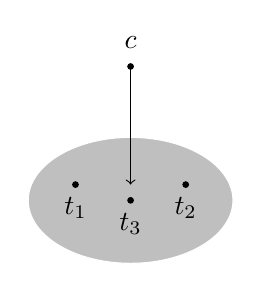
\begin{tikzpicture}
        \filldraw (0, 1.5) circle (1pt);
        \node at (0, 1.8) {$c$};
        
\filldraw[fill=gray!50, draw=white] (0, -0.2) ellipse (1.3 and 0.8);
        \filldraw (-0.7, 0) circle (1pt);
        \node at (-0.7, -0.3) {$t_1$};
        \filldraw (0.7, 0) circle (1pt);
        \node at (0.7, -0.3) {$t_2$};
        \filldraw (0, -0.2) circle (1pt);
        \node at (0, -0.5) {$t_3$};
        
    	\draw[->] (0, 1.5) -- (0, 0);
\end{tikzpicture}
\]

완비 코카테고리(cocomplete category)에서는 항상 쌍대곱(coproduct) $\coprod_{i \in I} t_i$를 구성할 수 있니다. 이 쌍대곱은 약한 종말 대상(weakly terminal object)인데, 이는 모든 $c$로부터 그것으로 가는 화살표가 있기 때문입니다. 이 화살표는 일부 $t_i$로 가는 화살표와 주입 $\iota_i \colon t_i \to \coprod_{j \in I} t_j$의 합성입니다.

약하게 종말 대상(weakly terminal object)이 주어진 경우, 우리는 (강한) 종말 대상(strongly terminal object)을 구성할 수 있습니. 우선 $\cat C$의 부분 범주(subcategory)인 $\cat T$의 대상을 $t_i$로 정의합니. $\cat T$ 내의 사상(Morphism)은 $\cat T$의 대상들 사이를 이동하는 $\cat C$ 내의 모든 사상입니. 이를 \index{full subcategory}\emph{충분한} 부분 범주(full subcategory)라 합니. 우리의 구성에 의해, $\cat T$는 작습니.

분명한 포함 함자(영문 용어: inclusion functor) $F$가 $\cat T$를 $\cat C$에 포함시킨다. 이 함자는 $\cat C$ 내에서 작은 도형을 정의한다. 이 도형의 쌍극한은 $\cat C$에서의 종점(terminal object)이라는 결과가 나온다.

반대로, 유사한 구성은 초기 객체(initial object)를 약 초기 집합(weakly initial set)의 극한(limit)으로 정의하는 데 사용할 수 있습니니다.

해의 집합이 가지는 이 성질은 Freyd의 쌍대 함자 정리(the Freyd's Adjoint Functor Theorem) 증명에서 유용할 것입니다.

\section{요네다 보조정리(Yoneda Lemma)}

한 범주 $\mathcal{C}$에서 집합의 범주로의 함자(functor)는 이 범주의 집합(Category of Sets)에서의 모델로 생각할 수 있습니다. 일반적으로 모델링(modeling)은 손실이 있는 과정입니다: 즉, 일부 정보를 버립니다. 상수 $\Set$ 값의 함자는 극단적인 예입니다: 이는 전체 범주를 단일 집합과 그 항등 함수(identity function)로 매핑합니다.

호옴 펑터(hom-functor)는 특정한 관점에서 범주(category)의 모델을 생성합니다. 예를 들어, 펑터 $\mathcal{C}(a, -)$는 $a$의 관점에서 $\mathcal{C}$의 전경을 제공합니다. 이는 $a$에서 나오는 모든 화살표들을 정돈된 패키지로 정리하고, 이러한 패키지들을 화살표들의 이미지들로 연결합니다. 이 모든 과정은 원래의 출발 범주의 구조에 따라 이루어집니다.

\[
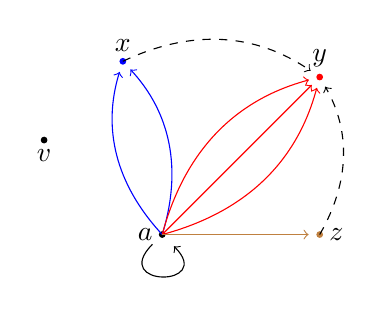
\begin{tikzpicture}
\def\ax{0}
\def\ay{0.5}
\def\xx{-0.5}
\def\xy{2.7}
\def\yx{2}
\def\yy{2.5}
\def\zx{2}
\def\zy{0.5}
\def\vx{-1.5}
\def\vy{1.7}
\filldraw[black] (\ax, \ay) circle (1 pt);
\node (a) at (\ax, \ay) {};
\node[left] at (\ax, \ay) {$a$};
\filldraw[blue] (\xx, \xy) circle (1 pt);
\node[above] at (\xx, \xy) {$x$};
\filldraw[red] (\yx, \yy) circle (1 pt);
\node[above] at (\yx, \yy) {$y$};
\filldraw[brown] (\zx, \zy) circle (1 pt);
\node[right] at (\zx, \zy) {$z$};
\filldraw[black] (\vx, \vy) circle (1 pt);
\node[below] at (\vx, \vy) {$v$};

\draw [->] (a) edge[out=225, in=315, loop] (a);

\draw[dashed] (\xx, \xy) edge[->, bend left, shorten > = 4 pt] (\yx, \yy);
\draw[dashed] (\zx, \zy) edge[->, bend right, shorten > = 4 pt] (\yx, \yy);

\draw[blue] (\ax, \ay) edge[->, bend left, shorten > = 4 pt] (\xx, \xy);
\draw[blue] (\ax, \ay) edge[->, bend right, shorten > = 4 pt] (\xx, \xy);

\draw[red] (\ax, \ay) edge[->, bend left, shorten > = 4 pt] (\yx, \yy);
\draw[red] (\ax, \ay) edge[->, bend right, shorten > = 4 pt] (\yx, \yy);
\draw[red] (\ax, \ay) edge[->, shorten > = 4 pt] (\yx, \yy);

\draw[brown] (\ax, \ay) edge[->, shorten > = 4 pt] (\zx, \zy);
\end{tikzpicture}
\hspace{80pt}여기서 $y$-좌표의 이동은\\
\hspace{80pt}교환 법칙(commutativity)으로부터\\
\hspace{80pt}결정되며 주어진
<|vq_3133|>
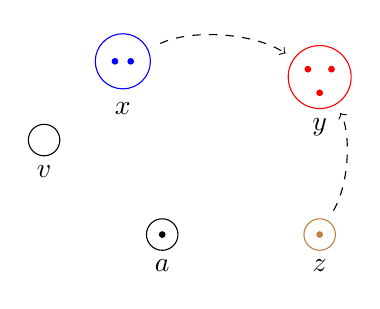
\begin{tikzpicture}
\def\ax{0}
\def\ay{0.5}
\def\xx{-0.5}
\def\xy{2.7}
\def\yx{2}
\def\yy{2.5}
\def\zx{2}
\def\zy{0.5}
\def\vx{-1.5}
\def\vy{1.7}
\def\sx{0.7}
\def\sy{1.6}

\node at (\sx, \sy) {$\Set$};

\draw[black] (\vx, \vy) circle (0.2);
\node[below] at (\vx, \vy - 0.2) {$v$};

\draw[black] (\ax, \ay) circle (0.2);
\filldraw[black] (\ax, \ay) circle (1 pt);
\node[below] at (\ax, \ay-0.2) {$a$};

\draw[blue] (\xx, \xy) circle (0.35);
\filldraw[blue] (\xx - 0.1, \xy) circle (1 pt);
\filldraw[blue] (\xx + 0.1, \xy) circle (1 pt);
\node[above] at (\xx, \xy - 0.8) {$x$};

\draw[red] (\yx, \yy) circle (0.4);
\filldraw[red] (\yx-0.15, \yy+0.1) circle (1 pt);
\filldraw[red] (\yx+0.15, \yy+0.1) circle (1 pt);
\filldraw[red] (\yx, \yy-0.2) circle (1 pt);
\node[below] at (\yx, \yy - 0.4) {$y$};

\draw[brown] (\zx, \zy) circle (0.2);
\filldraw[brown] (\zx, \zy) circle (1 pt);
\node[below] at (\zx, \zy - 0.2) {$z$};

\draw[dashed] (\xx, \xy) edge[->, bend left, shorten > = 15, shorten < = 15] (\yx, \yy);
\draw[dashed] (\zx, \zy) edge[->, bend right, shorten > = 15, shorten < = 10] (\yx, \yy);

\end{tikzpicture}
\]


어떤 관점들은 다른 것들보다 더 낫습니다. 예를 들어, 초기 객체(initial object)에서의 관점은 상당히 드뭅니다. 각각의 객체 $x$는 고유한 사상 $0 \to x$에 해당하는 단일 집합 $\cat C(0, x)$에 매핑됩니다.

터미널 오브젝트 관점에서 보면 더 흥미롭습니다: 이는 모든 오브젝트를 그들의 (글로벌) 원소 집합 $\cat C(1, x)$에 매핑합니다.

요네다 보조정리(Yoneda lemma)는 범주 이론(category theory)에서 가장 심오한 명제 중 하나로 여겨질 수도 있고, 가장 사소한 명제 중 하나로 여겨질 수도 있습니다. 심오한 버전부터 시작하겠습니다.

두 개의 $\mathcal{C}$ 모델을 $\mathbf{Set}$ 안에서 고려해 봅시다: 하나는 hom-함수자(hom-functor) $\mathcal{C}(a, -)$에 의해 주어진 것으로, 이는 $a$의 관점에서 본 $\mathcal{C}$의 전경(panoramic view)입니다; 또 다른 하나는 임의의 함수자(Functor) $F \colon \mathcal{C} \to \mathbf{Set}$에 의해 주어진 것입니다. 이들 사이의 자연 변환(natural transformation)은 한 모델을 다른 모델에 삽입합니다. 이러한 자연 변환들의 집합은 $a$에서 $F$의 값에 의해 완전히 결정됩니다.

자연 변환 집합은 함수자 범주(functor category) $[\mathcal{C}, \mathbf{Set}]$의 hom-집합(hom-set)이므로, 이것이 요네다 보조정리(Yoneda lemma)의 형식적 명제입니다:

\[ [\mathcal{C}, \mathbf{Set}]( \mathcal{C}(a, -), F) \cong F a \]

이것이 작동하는 이유는 이 정리에 관련된 모든 사상(mappings)이 범주 $\mathcal{C}$의 구조와 그 모형(structure of its models)의 구조를 보존해야 한다는 요구사항에 묶이기 때문입니다. 특히, 자연성 조건(naturality conditions)은 자연 변환(natural transformation)의 구성 요소들이 한 점에서 다른 점으로 전파되는 방식에 대해 매우 큰 제약을 부과합니다.

요네다 보조정리(Yoneda lemma)의 증명은 하나의 단일 항등 화살표로 시작하고 자연성(naturality)을 통해 이를 전체 범주(category)에 전파합니다.

여기 증명의 개요가 있습니다. 두 부분으로 구성됩니다: 먼저, 자연 변환(natural transformation)을 주어 $F a$의 한 원소를 구성합니다. 두 번째로, $F a$의 한 원소를 주어 해당 자연 변환을 구성합니다.

먼저, 왼쪽에 있는 임의의 요소를 선택합시다: 자연 변환(natural transformation) $\alpha$. 그것의 $x$에서의 구성 요소는 함수입니다:
\[ \alpha_x \colon \mathcal{C}(a, x) \to F x \]
이제 요네다 트릭(Yoneda trick)을 적용해 봅시다: $a$를 $x$로 대체합니다:
\[ \alpha_a \colon \mathcal{C}(a, a) \to F a \]
그리고 항등원 $id_a$를 $\mathcal{C}(a, a)$의 정규 원소로 선택합니다. 이는 집합 $F a$에서 원소 $\alpha_a (id_a)$를 제공합니다. 이는 자연 변환에서 집합 $F a$의 원소로의 한 방향의 매핑을 정의합니다.

$\cat C(a, -)$ 함자(hom-functor)의 그림을 보면, 그것이 $a$ 자체에 작용하는 결과는 항상 비어 있지 않은 집합임을 알 수 있읍니다. 만약 그것에서 $F$로의 자연 변환(natural transformation)이 존재한다면, 이는 $F a$도 비어 있지 않아야 함을 의미합니다.
\[
\begin{tikzpicture}
\def\ax{0}
\def\ay{0.5}
\def\xx{-0.5}
\def\xy{3.7}
\filldraw[black] (\ax, \ay) circle (1 pt);
\node (a) at (\ax, \ay) {};
\node[left] at (\ax, \ay) {$a$};
\filldraw[blue] (\xx, \xy) circle (1 pt);
\node[above] at (\xx, \xy) {$x$};

\draw [->] (a) edge[out=225, in=315, loop] (a);
\node[right] at (\ax + 0.3, \ay - 0.35) {$id_a$};

\draw[blue] (\ax, \ay) edge[->, "$h$", bend right, shorten > = 4 pt] (\xx, \xy);

\end{tikzpicture}
\hspace{80pt}여기서 $y$-좌표의 이동은\\
\hspace{80pt}교환 법칙(commutativity)으로부터\\
\hspace{80pt}결정되며 주어진
<|vq_3133|>
\begin{tikzpicture}

\def\ax{0}
\def\ay{0.5}
\def\xx{-0.5}
\def\xy{3.7}

\def\fax{3}
\def\fay{0.5}
\def\fxx{3 - 0.5}
\def\fxy{3.7}

\def\px{\fax - 0.3}
\def\hx{\xx + 0.35}
% C(a,a)
\draw[black] (\ax, \ay) circle (0.2);
\filldraw[black] (\ax, \ay) circle (1 pt);
\node[below] at (\ax, \ay-0.2) {$\cat C (a, a)$};
% C(a,x)
\draw[black] (\xx, \xy) ellipse (0.7 and 0.4);

\filldraw[blue] (\xx + 0.35, \xy) circle (1 pt);
\node[left, blue] at (\hx, \xy) {$h$};

\node[above] at (\xx, \xy - 1.1) {$\cat C (a, x)$};
\draw[dashed] (\hx, \xy) edge[->, "$\alpha_x$", shorten > = 4 pt] (\fxx, \fxy);

% F a
\draw[red] (\fax, \fay) ellipse (0.7 and 0.4);
\filldraw[red] (\px, \fay) circle (1 pt);
\node[right, red] at (\px, \fay) {$p$};
\node[right, red] at (\fax + 0.7, \fay) {$F a$};
\draw[dashed] (\ax, \ay) edge[->, "$\alpha_a$", shorten > = 3 pt] (\px, \fay);
% F x
\draw[red] (\fxx, \fxy) circle (0.4);
\filldraw[red] (\fxx, \fxy) circle (1 pt);
\node[right, red] at (\fxx + 0.35, \fxy) {$F x$};

\draw[blue] (\px, \fay) edge[->, "$F h$", bend right, shorten > = 12, shorten < = 12] (\fxx, \fxy);

\end{tikzpicture}
\]


이제 반대로 해보겠습니다. 집합 $F a$의 원소 $p$가 주어졌을 때 자연 변환(natural transformation) $\alpha$를 구성하고자 합니다. 먼저, $p$를 $\alpha_a$가 $id_a \in \cat C(a, a)$에서 작용하는 것으로 선택합니다.

이제 임의의 객체 $x$와 $\cat C(a, x)$의 임의의 원소를 봅시다. 그러한 원소는 어떤 사상(arrow) $h \colon a \to x$에 대응됩니다. 우리의 자연 변환은 그것을 $F x$의 원소에 매핑해야 합니다. 우리는 $F$를 사용하여 사상(arrow) $h$를 들어올림으로써 그것을 할 수 있습니다. 우리는 다음과 같은 함수를 얻습니다:
\[F h \colon F a \to F x \]
이를 $p$에 적용하고 $F x$의 요소를 얻을 수 있습니다. 이 요소는 $h$에 대한 $\alpha_x$의 작용으로 취합니다:
\[ \alpha_x h = (F h) p \]

요네다 보조정리의 동형사상(Isomorphism)은 $a$뿐만 아니라 $F$에서도 자연적입니다(Natural). 다시 말해, 함자 범주(Funcator category)에서 화살을 적용함으로써 함자 $F$에서 다른 함자 $G$로 ``이동''할 수 있습니다. 여기서 화살은 자연 변환(Natural transformation)입니다. 이것은 추상화의 수준에서 상당한 도약이지만, 함자성(Functoriality)과 자연성(Naturality)의 모든 정의는 객체가 함자이고 화살이 자연 변환인 함수 범주에서도 똑같이 잘 작동합니다.

\begin{exercise}
Fill in the gap in the proof when $F a$ is empty.
\end{exercise}
\begin{exercise}
Show that the mapping 
\[ \mathcal{C}(a, x) \to F x\]
defined above is a natural transformation. Hint: Vary $x$ using some $f \colon x \to y$.
\end{exercise}
\begin{exercise}
Show that the formula for $\alpha_x$ can be derived from the assumption that $\alpha_a (id_a) = p$ and the naturality condition. Hint: The lifting of $h$ by the hom-functor $\cat C(a, h)$ is given by post-composition.
\end{exercise}

\subsection{프로그래밍에서의 요네다 보조정리(Yoneda lemma)}

이제 사소한 부분을 다루겠습니다: 요네다 보조정리(Yoneda Lemma)의 증명은 직접적으로 Haskell 코드로 변환됩니다. 우리는 hom-함자(hom-functor) \hask{a->x}와 어떤 함자(functor) \hask{f} 사이의 자연 변환(natural transformation)의 타입(type)으로 시작하여, 이것이 \hask{f}가 \hask{a}에 작용하는 타입과 동등함을 보입니다.
\begin{haskell}
forall x. (a -> x) -> f x.   -- is isomorphic to (f a)
\end{haskell}
우리는 표준 요네다 트릭(Yoneda trick)을 사용하여 \hask{f a} 유형의 값을 생성합니다
\begin{haskell}
yoneda :: Functor f => (forall x. (a -> x) -> f x) -> f a
yoneda g = g id
\end{haskell}
다음은 역함수(낮은 매핑)에 대한 
\begin{haskell}
yoneda_1 :: Functor f => f a -> (forall x. (a -> x) -> f x)
yoneda_1 y = \h -> fmap h y
\end{haskell}

유형(type)와 집합(set)을 혼합하여 약간 속임수를 쓰고 있다는 점을 주의하십시오. 현재의 공식에서 요네다 보조정리(Yoneda lemma)는 $\mathbf{Set}$ 값을 가지는 함자(functor)와 함께 작동합니다. 다시 말해, 정확한 표현은 자체적으로 강화된(enriched) 범주에서 요네다 보조정리의 강화된 버전을 사용한다고 말해야 합니다.

요네다 보조정리는 프로그래밍에서 몇 가지 흥미로운 적용 사례가 있습니다. 예를 들어, 요네다 보조정리를 항등 함자에 적용하면 무슨 일이 일어나는지 생각해 봅시다. 우리는 타입 \hask{a} (항등 함자가 \hask{a}에 작용하는 경우)와의 동형(isomorphism)을 얻습니다.
\begin{haskell}
forall x. (a -> x) -> x
\end{haskell}
우리는 이를 모든 데이터 타입 \hask{a}을/를 고차 다형 함수로 대체할 수 있다는 것이라고 해석합니다. 이 함수는 또 다른 함수---핸들러(handler), 콜백(callback), 또는 \emph{연속체}(continuation)라고 불리는---를 인자로 받습니다.

이것은 값의 타입 \hask{a}을(를) 원격 서버에서 받아와야 할 때 분산 프로그래밍에서 많이 사용되는 표준 연속 전달 변환입니다. 또한 재귀 알고리즘을 꼬리 재귀 함수로 바꾸는 프로그램 변환으로도 유용합니다.

Continuation-passing style은(Continuation-passing style) 다루기 어렵습니다. 왜냐하면 continuations의(compositions) 구성이 매우 복잡하여, 이는 프로그래머들이 흔히 ``콜백 지옥''(callback hell)이라고 부르는 결과를 초래하기 때문입니다. 다행히도 continuations는(compositions) 하나의 모나드(monad)를 형성하며, 이는 그들의 구성을 자동화할 수 있음을 의미합니다.

\subsection{반변(contravariant) Yoneda 레마(lemma)}

몇 개의 화살표를 뒤집으면, 요네다 보조정리(Yoneda lemma)는 반변 함자(contravariant functors)에도 적용할 수 있습니다. 이는 반변 함자 $\mathcal{C}(-, a)$와 반변 함자 $F$ 사이의 자연 변환(natural transformations)에서 작동합니다.

\[ [\mathcal{C}^{op}, \mathbf{Set}]( \mathcal{C}(-, a), F) \cong F a \]

이는 매핑(mapping)의 Haskell 구현입니다:
\begin{haskell}
coyoneda :: Contravariant f => (forall x. (x -> a) -> f x) -> f a
coyoneda g = g id
\end{haskell}
그리고 이것이 역변환(inverse transformation)이다:
\begin{haskell}
coyoneda_1 :: Contravariant f => f a -> (forall x. (x -> a) -> f x)
coyoneda_1 y = \h -> contramap h y
\end{haskell}

\section{요네다 매장(Yoneda Embedding)}

폐쇄 범주(closed category)에서, 우리는 hom-집합(hom-sets)의 대체물로서 지수 객체(exponential objects)를 가집니다. 이는 집합의 범주(category of sets)에서 명백하게 나타나는 일로, hom-집합이 집합이기 때문에 자동적으로 객체가 됩니다.

하지만 범주의 범주인 $\mathbf{Cat}$에서는 hom-집합(hom-sets)이 \emph{함자들(functors)}의 집합입니다. 그리고 이것들이 객체들로 승격될 수 있다는 것이 즉시 명백하지는 않습니다---즉, 범주들입니다. 하지만, 우리가 본 것처럼, 그것들은 가능합니다! 어떤 두 범주 사이의 함자들은 하나의 함자 \emph{범주(category)}를 형성합니다.

그 때문에, 펑터(functor) 또한 함수(function)를 커리하는 것처럼 커리할 수 있습니다. 곱 카테고리에서의 펑터는 펑터를 반환하는 펑터로 볼 수 있습니다. 다시 말해, $\mathbf{Cat}$은 닫힌 (대칭) 모노이드 카테고리입니다.

특히, 우리는 hom-펑터(hom-functor) $\mathcal{C}(a, b)$에 커링(currying)을 적용할 수 있습니다. 이는 프로펑터(profunctor)로, 곧 곱 카테고리에서 오는 펑터입니다.
\[ \mathcal{C}^{op} \times \mathcal{C} \to  \mathbf{Set} \]
하지만 이 또한 첫 번째 인자 $a$에서 반변함자(contravariant functor)입니다. 모든 $a \in \mathcal{C}^{op}$에 대해, 이는 함자 범주 $ [\mathcal{C},  \mathbf{Set}] $의 객체인 함자 $\mathcal{C}(a, -)$를 생성합니다. 이를 다음과 같이 쓸 수 있습니다:
\[ \mathcal{C}^{op} \to [\mathcal{C},  \mathbf{Set}] \]
대신, $b$에 집중하여 반변함수자(contravariant functor) $\mathcal{C}(-, b)$를 얻을 수 있습니다. 이 매핑(mapping)은 다음과 같이 쓸 수 있습니다.
\[ \mathcal{C} \to [\mathcal{C}^{op},  \mathbf{Set}] \]
두 사상은 모두 함자적(functorial)입니다. 이는 예를 들어, $\mathcal{C}$의 화살(arrow)이 $[\mathcal{C}^{op}, \mathbf{Set}]$에서 자연 변환(natural transformation)으로 사상됨을 의미합니다.

이러한 $\mathbf{Set}$ 값을 가지는 함자 범주(functor categories)는 매우 흔해서 특별한 이름이 있습니다. $[\mathcal{C}^{op},  \mathbf{Set}]$에 있는 함자를 \index{presheaves}\emph{전단사(presheaves)}라고 하며, $[\mathcal{C},  \mathbf{Set}]$에 있는 함자를 \index{co-presheaves}\emph{공전단사(co-presheaves)}라고 합니다. (이 이름들은 대수적 위상수학(algebraic topology)에서 유래했습니다.)

다음 호멤 함자(hom-functor)를 읽는 데 집중해 봅시다:
\[ \mathcal{Y} \colon \mathcal{C} \to [\mathcal{C}^{op},  \mathbf{Set}] \]
객체 $x$를 받아서 프리쉬프(presheaf)로 매핑합니다
\[ \mathcal Y_x = \mathcal{C}(-, x) \]
$x$의 모든 가능한 방향에서 본 $x$의 모든 관점의 총체로 시각화될 수 있습니다.

화살의 동작도 다시 검토해 봅시다. 함자(functor) $\mathcal{Y}$는 화살 $f \colon x \to y$를 전단사 사상의 매핑으로 들어올립니다:
\[ \alpha \colon \mathcal{C}(-, x) \to \mathcal{C}(-, y) \]
이 자연 변환의 한 성분(component) $z$에서의 성분은 hom-집합(hom-sets)들 사이의 함수입니다:
\[ \alpha_z \colon \mathcal{C}(z, x) \to \mathcal{C}(z, y) \]
단순히 후합성 $(f \circ -)$으로 구현됩니다.

이러한 함자 $\mathcal{Y}$는 준층 범주에서 $\mathcal{C}$의 모형을 생성하는 것으로 생각할 수 있습니. 하지만 이것은 평범한 모형이 아닙니다---한 범주를 다른 범주 안에 \emph{매장(embedding)}하는 것입니다. 이 특정한 경우는 \emph{요네다 매장(Yoneda embedding)}이라고 하며, 함자 $\mathcal{Y}$는 \index{Yoneda functor}\emph{요네다 함자(Yoneda functor)}라고 합니다.

우선, 모든 $\mathcal{C}$의 객체는 $[\mathcal{C}^{op},  \mathbf{Set}]$에서 서로 다른 객체(프리쉬프(presheaf))에 대응됩니다. 이는 \index{injection}\emph{객체에 대하여 단사적(injective)}이라고 합니다. 하지만 그것이 전부가 아닙니다: $\mathcal{C}$의 모든 사상 또한 서로 다른 사상에 대응됩니다. 이는 삽입 함자가 \index{faithful functor}\emph{충실하다(faithful)}고 합니다. 그것만으로도 충분하지 않다면, 호셋(hom-set)의 대응 역시 \index{surjection}전사적(surjective)이며, 이는 $[\mathcal{C}^{op},  \mathbf{Set}]$의 객체들 간의 모든 사상이 $\mathcal{C}$에서 온 사상임을 의미합니다. 이는 그 함자가 \index{full functor}\emph{완전하다(full)}고 합니다. 종합하면, 그 삽입은 \emph{완전 충실합니다(fully faithful)}.

후자의 사실은 요네다 보조정리(Yoneda lemma)의 직접적인 결과입니다. 우리는 다음을 알고 있습니다. 어떤 함자(functor) $F \colon \mathcal{C}^{op} \to \mathbf{Set}$에 대해서, 다음과 같은 자연 동형(natural isomorphism)이 있습니다:

\[ [\mathcal{C}^{op}, \mathbf{Set}]( \mathcal{C}(-, x), F) \cong F x \]
특히, 또 다른 hom-펑터 $\mathcal{C}(-, y)$를 $F$ 대신 대체할 수 있습니다:
\[ [\mathcal{C}^{op}, \mathbf{Set}]( \mathcal{C}(-, x), \mathcal{C}(-, y)) \cong \mathcal{C}(x, y)\]
왼쪽은 전도함수 범주(presheaf category)에서의 hom-집합(hom-set)이고, 오른쪽은 $\mathcal{C}$에서의 hom-집합입니다. 이들은 동형(isomorphic)이므로 포함 함수가 완전충만함(fully faithful)을 증명합니다.

이 동형사상(isomorphism)을 좀 더 자세히 살펴보겠습니다. 오른쪽 집합 $\mathcal{C}(x, y)$의 원소, 즉 화살표 $f$를 택해봅시다. 이 동형사상은 이를 각 $z$에서의 성분이 함수인 자연 변환으로 매핑합니다:
\[ \mathcal{C}(z, x) \to \mathcal{C}(z, y) \]
이 사상은 $(f \circ -)$의 사후 구성(post-composition)으로 구현됩니다.

Haskell에서는 다음과 같이 작성합니다:
\begin{haskell}
toNat :: (x -> y) -> (forall z. (z -> x) -> (z -> y))
toNat f = \h -> f . h 
\end{haskell}
사실, 이 구문도 작동합니다:
\begin{haskell}
toNat f = (f . )
\end{haskell}
역함수는:
\begin{haskell}
fromNat :: (forall z. (z -> x) -> (z -> y)) -> (x -> y)
fromNat alpha = alpha id
\end{haskell}
(요네다(Yoneda) 트릭을 다시 사용하는 것을 주목하세요.)

이 동형사상은 항등원(identity)을 항등원으로, 합성(composition)을 합성으로 매핑합니다. 이는 사후 합성(post-composition)으로 구현되기 때문이며, 사후 합성은 항등원과 합성을 모두 보존합니다. 우리는 동형사상에 관한 장에서 이를 보았습니다.
\[ ((f \circ g) \circ -) = (f \circ -) \circ (g \circ -) \]

구성이와 항등원을 보존하기 때문에, 이 동형사상(isomorphism)은 또한 \emph{동형사상}(isomorphisms)을 보존합니다. 따라서 만약 $x$가 $y$와 동형사상이라면, 프리쉬브(presheaves) $ \mathcal{C}(-, x)$와 $ \mathcal{C}(-, y)$ 또한 동형사상이며, 그 역도 성립합니다.

이것이 바로 이전 장들에서 수많은 동형사상을 증명하기 위해 우리가 계속 사용해온 결과입니다.

\section{표현 가능 함자(Representable Functors)}

대상은 co-프리셰이프 카테고리의 functor들이며, 이는 $\mathcal{C}$의 대상들에 집합들을 할당합니다. 이러한 functor들 중 일부는 참조 대상 $a$를 선택하고, 모든 대상 $x$에 대해 그들의 hom-집합(hom-sets) $\mathcal{C}(a, x)$을 할당함으로써 작동합니다:
\[ F x = \cat C(a, x) \]
그러한 함수자(functor)와 그것들과 동형인 모든 함수자를 \emph{표현 가능하다}(representable)고 합니다. 전체 함수자는 단일 객체 $a$로 ``표현됩니다''.

닫힌 범주(closed category)에서는, 객체 $x$에 $x^a$의 원소 집합을 할당하는 함자(functor)는 $a$에 의해 표현됩니다. 왜냐하면 $x^a$의 원소 집합은 $\mathcal{C}(a, x)$와 동형이기 때문입니다:
\[\mathcal{C}(1, x^a) \cong \mathcal{C}(1 \times a, x) \cong \mathcal{C} (a, x)\]

이와 같이 보면, 표현하는 객체 $a$는 함자(functor)의 로그(logarithm)와 같다.

유사성은 더 깊어집니다: 마치 곱셈의 로그가 로그들의 합인 것처럼, 곱 데이터 타입(product data type)을 나타내는 객체는 합입니다. 예를 들어, 곱을 사용하여 인수를 제곱하는 functor, $F x = x \times x$ 는 $2$로 표현됩니다. 이는 합 $1 + 1$ 입니다. 실제로, 우리는 이전에 $x \times x \cong x^2$임을 보았습니다.

표현 가능 함자(representable functors)는 $\mathbf{Set}$ 값을 가지는 함수자의 범주에서 매우 특별한 역할을 합니다. 요네다 매장은 $\mathcal{C}$의 객체를 표현 가능 전층으로 매핑함을 주목하십시오. 그것은 객체 $x$를 $x$에 의해 표현되는 전층으로 매핑합니다:

\[  \mathcal{Y} \colon x \mapsto \mathcal{C}(-, x) \]

전체 범주 $\mathcal{C}$, 객체(objects)와 사상(morphisms)을 표현 가능 함자(representable functors)로서 전단사 사상(embedding)된 전형(precisely) 범주 안에서 찾을 수 있습니.  
질문은, 전형 범주에는 표현 가능 함자 간의 ``사이에'' 무엇이 더 있나요?

마치 유리수( rational numbers) 가 실수(real numbers) 사이에서 조밀(dense)한 것처럼, 표현 가능 범주(representables) 도 (공)프리쉬브((co-) presheaves) 사이에서 ``조밀''합니다. 모든 실수는 유리수로 근사화될 수 있습니다. 모든 프리쉬브(presheaf)는 표현 가능 범주의 콜리밋(colimit)이며, 모든 공-프리쉬브(co-presheaf)는 리밋(limit)입니다. 이 주제에 대해서는 (공-) 끝((co-) ends)을 논할 때 다시 다루겠습니다.

\begin{exercise}
Describe limits and colimits as representing objects. What are the functors they represent?
\end{exercise}
\begin{exercise}
Consider a \emph{singleton functor} $F \colon \cat C \to \Set$ that assigns to each object $c$ a singleton set $\{c\}$ that contains just that object (that is, a different singleton for every object). Define the action of $F$ on arrows. Show that $F$ being representable is equivalent to $\cat C$ having an initial object.
\end{exercise}

\subsection{추측 게임(The guessing game)}

대상들이 다른 대상들과 상호작용하는 방식에 의해 설명될 수 있다는 아이디어는 때때로 상상의 추측 게임을 통해 설명되기도 합니다. 한 범주론(category theorist) 학자가 범주에서 비밀 대상을 선택하고, 다른 학자가 그것이 어떤 대상인지를 (물론 동형사상(isomorphism)까지 포함해) 추측해야 합니다.

추측자는 객체들을 가리키고, 이들을 비밀 객체에 대한 ``탐침(probe)''으로 사용할 수 있습니니다. 상대자는 매번 답을 해야 하는데: 이는 탐침 객체 $a$ 에서 비밀 객체 $x$ 까지의 화살표 집합입니다. 이는 물론 동형 집합(hom-set) $\mathcal{C}(a, x)$ 입니다.

이 답변들의 총체는 상대방이 부정행위를 하지 않는 한 프리쉬프 $F \colon \mathcal{C}^{op} \to \mathbf{Set}$를 정의할 것이고, 그들이 숨기고 있는 객체는 그 표현 객체입니다.

하지만 우리가 그들이 속이지 않는다는 것을 어떻게 알 수 있을까요? 이를 테스트하려면 화살(arrow)에 대한 질문을 할 수 있어야 합니다. 우리가 선택한 각 화살마다 그들은 우리에게 두 집합 사이의 함수(function)를 제공해야 합니다---우리가 화살의 끝점으로 주어진 집합들이 바로 그것입니다. 그 다음 우리는 모든 항등 화살(identity arrows)이 항등 함수(identity functions)로 매핑되는지, 화살의 합성(compositions)이 함수의 합성으로 매핑되는지 확인할 수 있습니다. 다시 말해, 우리가 $F$가 함자(functor)임을 확인할 수 있게 됩니다.

그러나 충분히 영리한 상대는 여전히 우리를 속일 수 있읍니다. 그들이 우리에게 보여주는 사전층(presheaf)는 환상적인 객체를 묘사할 수 있으며---그들의 상상의 산물일 수 있으며---우리는 이를 구분할 수 없을 것입니니다. 그러한 상상의 객체가 실제 객체만큼 흥미로운 경우가 많다는 것이 밝혀졌습니다.

\subsection{프로그래밍에서 표현가능한 함자(Representable functors)}

Haskell에서 우리는 다음 두 가지 함수를 사용하여 대응함을 증명하는 표현 가능한 펑터(representable functors)의 클래스를 정의합니다: \hask{tabulate} 함수는 함수를 조회 테이블로 바꾸며, \hask{index} 함수는 표기 타입 \hask{Key}를 사용하여 그 내부를 인덱싱합니다.

\begin{haskell}
class Representable f where
  type Key f :: Type
  tabulate :: (Key f -> a) -> f a
  index    :: f a -> (Key f -> a)
\end{haskell}

대수적 데이터 타입(Algebraic data types) 중 합(sums)을 사용하는 것들은 표현될 수 없습니다---합의 로그를 취하는 공식은 존재하지 않습니다. 리스트 타입(List type)은 합으로 정의되므로, 이는 표현될 수 없습니다.

그러나, 무한 스트림은. 개념적으로, 이러한 스트림은 무한 튜플과 같으며, 이는 기술적으로는 곱(product)입니다. 스트림은 자연수의 타입으로 표현됩니다. 다시 말해, 무한 스트림은 자연수로부터의 매핑(mapping)과 동일합니다.
\begin{haskell}
data Stream a = Stm a (Stream a)
\end{haskell}
여기 개체(instance) 정의가 있습니다:
\begin{haskell}
instance Representable Stream where
  type Key Stream = Nat
  tabulate g = tab Z
    where
      tab n = Stm (g n) (tab (S n))
  index stm = \n -> ind n stm
    where
      ind Z (Stm a _) = a
      ind (S n) (Stm _ as) = ind n as
\end{haskell}
표현 가능한 타입(Representable types)은 함수의 메모이제이션(memoization)을 구현하는 데 유용합니다.

\begin{exercise}
Implement the \hask{Representable} instance for \hask{Pair}:
\begin{haskell}
data Pair x = Pair x x
\end{haskell}
\end{exercise}

\begin{exercise}
Is the constant functor that maps everything to the terminal object representable? Hint: what's the logarithm of 1?

In Haskell, such a functor could be implemented as:
\begin{haskell}
data Unit a = U
\end{haskell}
이를 위해 \hask{Representable}의 인스턴스를 구현합니다.
\end{exercise}

\begin{exercise}
The list functor is not representable. But can it be considered a sum or representables?
\end{exercise}

\section{2-범주 $\mathbf{Cat}$ }

카테고리의 카테고리인 $\mathbf{Cat}$에서는, hom-집합들(hom-sets)은 단지 집합이라고만 볼 수 없습니다. 각각은 함자 카테고리(functor category)로 승격될 수 있으며, 자연 변환(natural transformations)이 화살표(arrows)의 역할을 합니다. 이러한 구조를 2-카테고리(2-category)라고 부릅니다.

2-범주의 언어에서, 객체는 0-셀(cell)이라 불리며, 객체 사이의 화살표는 1-셀이라 불립니다, 그리고 화살표들 사이의 화살표는 2-셀이라 불립니다.

그 그림의 명백한 일반화는 3-세포(3-cells)를 2-세포(2-cells) 사이로 이어지는 것으로 간주하는 것입니다. $n$-카테고리($n$-category)는 $n$번째 레벨까지 이어지는 세포들을 갖습니다.

그러나 왜 화살표가 끝까지 이어지지 않는가? 무한 범주($\infty$-categories)에 들어가 보자. 이는 호기심에서 끝나지 않고 실용적인 응용을 가지고 있습니니다. 예를 들어, $\infty$-범주는 대수적 위상수학(algebraic topology)에서 점, 점 사이의 경로, 경로가 훑고 지나가는 표면, 표면이 훑고 지나가는 부피 등을 묘사하는데 사용됩니니다. 그리고 계속해서 무한히 이어집니니다.

\section{유용한 공식들}
\begin{itemize}
\item Yoneda lemma for covariant functors:
\[ [\mathcal{C}, \mathbf{Set}]( \mathcal{C}(a, -), F) \cong F a \]
\item Yoneda lemma for contravariant functors:
\[ [\mathcal{C}^{op}, \mathbf{Set}]( \mathcal{C}(-, a), F) \cong F a \]
\item Corollaries to the Yoneda lemma:
\begin{align*}
 [\mathcal{C}, \mathbf{Set}]( \mathcal{C}(x, -), \mathcal{C}(y, -)) &\cong \mathcal{C}(y, x) \\
 [\mathcal{C}^{op}, \mathbf{Set}]( \mathcal{C}(-, x), \mathcal{C}(-, y)) &\cong \mathcal{C}(x, y)
\end{align*}

\end{itemize}

\end{document}